% A LaTeX template for MSc Thesis submissions to 
% Politecnico di Milano (PoliMi) - School of Industrial and Information Engineering
%
% S. Bonetti, A. Gruttadauria, G. Mescolini, A. Zingaro
% e-mail: template-tesi-ingind@polimi.it
%
% Last Revision: October 2021
%
% Copyright 2021 Politecnico di Milano, Italy. NC-BY

\documentclass{Configuration_Files/PoliMi3i_thesis}

%------------------------------------------------------------------------------
%	REQUIRED PACKAGES AND  CONFIGURATIONS
%------------------------------------------------------------------------------

% CONFIGURATIONS
\usepackage{parskip} % For paragraph layout
\usepackage{setspace} % For using single or double spacing
\usepackage{emptypage} % To insert empty pages
\usepackage{multicol} % To write in multiple columns (executive summary)
\setlength\columnsep{15pt} % Column separation in executive summary
\setlength\parindent{0pt} % Indentation
\raggedbottom  

% PACKAGES FOR TITLES
\usepackage{titlesec}
% \titlespacing{\section}{left spacing}{before spacing}{after spacing}
\titlespacing{\section}{0pt}{3.3ex}{2ex}
\titlespacing{\subsection}{0pt}{3.3ex}{1.65ex}
\titlespacing{\subsubsection}{0pt}{3.3ex}{1ex}
\usepackage{color}

% PACKAGES FOR LANGUAGE AND FONT
\usepackage[english]{babel} % The document is in English  
\usepackage[utf8]{inputenc} % UTF8 encoding
\usepackage[T1]{fontenc} % Font encoding
\usepackage[11pt]{moresize} % Big fonts

% PACKAGES FOR IMAGES
\usepackage{graphicx}
\usepackage{transparent} % Enables transparent images
\usepackage{eso-pic} % For the background picture on the title page
\usepackage{subfig} % Numbered and caption subfigures using \subfloat.
\usepackage{tikz} % A package for high-quality hand-made figures.
\usetikzlibrary{}
\graphicspath{{./Images/}} % Directory of the images
\usepackage{caption} % Coloured captions
\usepackage{xcolor} % Coloured captions
\usepackage{amsthm,thmtools,xcolor} % Coloured "Theorem"
\usepackage{float}

% STANDARD MATH PACKAGES
\usepackage{amsmath}
\usepackage{amsthm}
\usepackage{amssymb}
\usepackage{amsfonts}
\usepackage{bm}
\usepackage[overload]{empheq} % For braced-style systems of equations.
\usepackage{fix-cm} % To override original LaTeX restrictions on sizes

% PACKAGES FOR TABLES
\usepackage{tabularx}
\usepackage{longtable} % Tables that can span several pages
\usepackage{colortbl}

% PACKAGES FOR ALGORITHMS (PSEUDO-CODE)
\usepackage{algorithm}
\usepackage{algorithmic}

% PACKAGES FOR REFERENCES & BIBLIOGRAPHY
\usepackage[colorlinks=true,linkcolor=black,anchorcolor=black,citecolor=black,filecolor=black,menucolor=black,runcolor=black,urlcolor=black]{hyperref} % Adds clickable links at references
\usepackage{cleveref}
\usepackage[square, numbers, sort&compress]{natbib} % Square brackets, citing references with numbers, citations sorted by appearance in the text and compressed
\bibliographystyle{abbrvnat} % You may use a different style adapted to your field

% OTHER PACKAGES
\usepackage{pdfpages} % To include a pdf file
\usepackage{afterpage}
\usepackage{lipsum} % DUMMY PACKAGE
\usepackage{fancyhdr} % For the headers
\fancyhf{}

\usepackage{graphicx}
\usepackage{tocloft}  
\usepackage{titling}  
\usepackage{booktabs} 
\usepackage{tabularx}  
\usepackage{geometry} 
\usepackage{longtable}
\usepackage{multirow}
\usepackage{todonotes}
\usepackage{listings}
\usepackage{xcolor}
\usepackage{amsmath} 
\usepackage[colorlinks=true, linkcolor=black, urlcolor=black, citecolor=black, filecolor=black]{hyperref}

%PlantUml package
\usepackage{plantuml}


% Define colors for custom Alloy highlighting
\definecolor{commentgreen}{rgb}{0,0.6,0}
\definecolor{keywordblue}{rgb}{0.13,0.13,1}
\definecolor{stringred}{rgb}{0.8,0,0}
\definecolor{numberpurple}{rgb}{0.58,0,0.83}

% Define Alloy language syntax highlighting
\lstdefinelanguage{Alloy}{
    keywords={sig, extends, fact, pred, fun, run, assert, check, some, all, no, one, lone, abstract, disj, module, open, set},
    keywordstyle=\color{keywordblue}\bfseries,
    comment=[l]{//},              % comment style
    commentstyle=\color{commentgreen},
    stringstyle=\color{stringred},
    morestring=[b]",              % strings are in quotes
    sensitive=true,               % case sensitive
    morekeywords={in, and, or, not, implies, iff}, % Alloy-specific keywords
    morecomment=[s]{/*}{*/},      % block comment style
    literate={0}{{\textcolor{numberpurple}{0}}}{1}%
             {1}{{\textcolor{numberpurple}{1}}}{1}%
             {2}{{\textcolor{numberpurple}{2}}}{1}%
             {3}{{\textcolor{numberpurple}{3}}}{1}%
             {4}{{\textcolor{numberpurple}{4}}}{1}%
             {5}{{\textcolor{numberpurple}{5}}}{1}%
             {6}{{\textcolor{numberpurple}{6}}}{1}%
             {7}{{\textcolor{numberpurple}{7}}}{1}%
             {8}{{\textcolor{numberpurple}{8}}}{1}%
             {9}{{\textcolor{numberpurple}{9}}}{1}%
}

\lstset{
    language=Alloy,
    basicstyle=\ttfamily\footnotesize,
    numbers=left,
    numberstyle=\tiny\color{gray},
    stepnumber=1,
    breaklines=true,
    showstringspaces=false,
    frame=single,
    caption=Alloy Example,
    label=code:alloy_example,
}

\setlength{\cftbeforesecskip}{10pt}


% Input of configuration file. Do not change config.tex file unless you really know what you are doing. 
% Define blue color typical of polimi
\definecolor{bluepoli}{cmyk}{0.4,0.1,0,0.4}

% Custom theorem environments
\declaretheoremstyle[
  headfont=\color{bluepoli}\normalfont\bfseries,
  bodyfont=\color{black}\normalfont\itshape,
]{colored}

% Set-up caption colors
\captionsetup[figure]{labelfont={color=bluepoli}} % Set colour of the captions
\captionsetup[table]{labelfont={color=bluepoli}} % Set colour of the captions
\captionsetup[algorithm]{labelfont={color=bluepoli}} % Set colour of the captions

\theoremstyle{colored}
\newtheorem{theorem}{Theorem}[chapter]
\newtheorem{proposition}{Proposition}[chapter]

% Enhances the features of the standard "table" and "tabular" environments.
\newcommand\T{\rule{0pt}{2.6ex}}
\newcommand\B{\rule[-1.2ex]{0pt}{0pt}}

% Pseudo-code algorithm descriptions.
\newcounter{algsubstate}
\renewcommand{\thealgsubstate}{\alph{algsubstate}}
\newenvironment{algsubstates}
  {\setcounter{algsubstate}{0}%
   \renewcommand{\STATE}{%
     \stepcounter{algsubstate}%
     \Statex {\small\thealgsubstate:}\space}}
  {}

% New font size
\newcommand\numfontsize{\@setfontsize\Huge{200}{60}}

% Title format: chapter
\titleformat{\chapter}[hang]{
\fontsize{50}{20}\selectfont\bfseries\filright}{\textcolor{bluepoli} \thechapter\hsp\hspace{2mm}\textcolor{bluepoli}{|   }\hsp}{0pt}{\huge\bfseries \textcolor{bluepoli}
}

% Title format: section
\titleformat{\section}
{\color{bluepoli}\normalfont\Large\bfseries}
{\color{bluepoli}\thesection.}{1em}{}

% Title format: subsection
\titleformat{\subsection}
{\color{bluepoli}\normalfont\large\bfseries}
{\color{bluepoli}\thesubsection.}{1em}{}

% Title format: subsubsection
\titleformat{\subsubsection}
{\color{bluepoli}\normalfont\large\bfseries}
{\color{bluepoli}\thesubsubsection.}{1em}{}

% Shortening for setting no horizontal-spacing
\newcommand{\hsp}{\hspace{0pt}}

\makeatletter
% Renewcommand: cleardoublepage including the background pic
\renewcommand*\cleardoublepage{%
  \clearpage\if@twoside\ifodd\c@page\else
  \null
  \AddToShipoutPicture*{\BackgroundPic}
  \thispagestyle{empty}%
  \newpage
  \if@twocolumn\hbox{}\newpage\fi\fi\fi}
\makeatother

%For correctly numbering algorithms
\numberwithin{algorithm}{chapter}


%----------------------------------------------------------------------------
%	NEW COMMANDS DEFINED
%----------------------------------------------------------------------------

% EXAMPLES OF NEW COMMANDS
\newcommand{\bea}{\begin{eqnarray}} % Shortcut for equation arrays
\newcommand{\eea}{\end{eqnarray}}
\newcommand{\e}[1]{\times 10^{#1}}  % Powers of 10 notation

%----------------------------------------------------------------------------
%	ADD YOUR PACKAGES (be careful of package interaction)
%----------------------------------------------------------------------------

%----------------------------------------------------------------------------
%	ADD YOUR DEFINITIONS AND COMMANDS (be careful of existing commands)
%----------------------------------------------------------------------------

%----------------------------------------------------------------------------
%	BEGIN OF YOUR DOCUMENT
%----------------------------------------------------------------------------

\begin{document}

\fancypagestyle{plain}{%
\fancyhf{} % Clear all header and footer fields
\fancyhead[RO,RE]{\thepage} %RO=right odd, RE=right even
\renewcommand{\headrulewidth}{0pt}
\renewcommand{\footrulewidth}{0pt}}

%----------------------------------------------------------------------------
%	TITLE PAGE
%----------------------------------------------------------------------------

\pagestyle{empty} % No page numbers
\frontmatter % Use roman page numbering style (i, ii, iii, iv...) for the preamble pages

\puttitle{
    title=Design Document, % Title of the thesis
    nameA=Giovanni Vaccarino, % Author Name and Surname
    nameB=Vittorio Palladino, % Author Name and Surname
    nameC=Nicolò Vacis, % Author Name and Surname
    course=Computer Science and Engineering, % Study Programme (in Italian)
    academicyear={2024{-}25},  % Academic Year
} % These info will be put into your Title page 

%----------------------------------------------------------------------------
%	LIST OF CONTENTS/FIGURES/TABLES/SYMBOLS
%----------------------------------------------------------------------------

% TABLE OF CONTENTS
\thispagestyle{empty}
\tableofcontents % Table of contents 
\thispagestyle{empty}
\cleardoublepage

%-------------------------------------------------------------------------
%	THESIS MAIN TEXT
%-------------------------------------------------------------------------
% In the main text of your thesis you can write the chapters in two different ways:
%
%(1) As presented in this template you can write:
%    \chapter{Title of the chapter}
%    *body of the chapter*
%
%(2) You can write your chapter in a separated .tex file and then include it in the main file with the following command:
%    \chapter{Title of the chapter}
%    \input{chapter_file.tex}
%
% Especially for long thesis, we recommend you the second option.

\addtocontents{toc}{\vspace{2em}} % Add a gap in the Contents, for aesthetics
\mainmatter % Begin numeric (1,2,3...) page numbering

% --------------------------------------------------------------------------
% NUMBERED CHAPTERS % Regular chapters following
% --------------------------------------------------------------------------

\chapter{Introduction}
\section{Scope}

The S\&C platform is a web-based solution intended to support:
\begin{itemize}
    \item \textbf{Students} in finding internships suited to their skills and aspirations, allowing them to submit CVs and receive tailored recommendations.
    \item \textbf{Companies} in listing internship opportunities and identifying candidates based on skills and profiles.
    \item \textbf{Universities} in overseeing internships, tracking progress, addressing complaints, and ensuring the quality of internships.
\end{itemize}
The platform enables interaction among these groups, handling tasks like matching candidates with internships, interview scheduling, feedback collection, and assessing internship effectiveness. The platform is built to scale across universities, supporting thousands of users.

\section{Definitions, Acronyms, Abbreviations}

\subsection{Definitions}
\begin{itemize}
    \item \textbf{Slug}: A human-readable and URL-friendly string (typically lowercase ASCII characters) that uniquely identifies a specific resource. It is commonly used in URLs but may also serve as an identifier for resources, like internship listings or profiles, within the S\&C platform.
    \item \textbf{S\&C Repository Slug}: A slug in the format `<repository owner>/<repository name>` that uniquely identifies a project repository on the S\&C platform or external GitHub repositories associated with student or company projects.
\end{itemize}

\subsection{Acronyms}
\begin{itemize}
    \item \textbf{S\&C}: Students\&Companies platform
    \item \textbf{API}: Application Programming Interface
    \item \textbf{CV}: Curriculum Vitae
    \item \textbf{GDPR}: General Data Protection Regulation
    \item \textbf{GH}: GitHub
    \item \textbf{SSO}: Single Sign-On
    \item \textbf{UUID}: Universal Unique Identifier
    \item \textbf{DB}: Database
    \item \textbf{DBMS}: Database Management System
    \item \textbf{RPC}: Remote Procedure Call
    \item \textbf{REST}: Representational State Transfer
    \item \textbf{SPA}: Single Page Application
    \item \textbf{CDN}: Content Delivery Network
\end{itemize}

\subsection{Abbreviations}
\begin{itemize}
    \item \textbf{e.g.}: For example
    \item \textbf{repo}: Repository
    \item \textbf{ID}: Identifier
\end{itemize}

\section{Revision History}
\begin{table}[h!]
\centering
\begin{tabular}{|c|c|l|}
\hline
\textbf{Version} & \textbf{Date} & \textbf{Description} \\ \hline
1.0 & January 7, 2024 & Initial release \\ \hline
\end{tabular}
\end{table}


\section{Reference Documents}
\begin{itemize}
    \item Specification document: "Assignment RDD AY 2023-2024"
    \item UML official specification: \url{https://www.omg.org/spec/UML/}
    \item Requirements Analysis and Specification Document: "RASD"
\end{itemize}

\section{Document Structure}
The document is organized into the following sections:
\begin{itemize}
    \item \textbf{Section 1: Introduction} - Provides an overview of the problem and the system's scope. It also includes definitions, acronyms, abbreviations, and a revision history to track document versions and modifications.
    \item \textbf{Section 2: Architectural Design} - Describes the system architecture, starting with a high-level overview of design choices, followed by detailed component and deployment views, including server, client, and data components (DB schemas). This section also presents sequence diagrams to illustrate the system’s runtime view and includes information on component interfaces, design styles, and architectural patterns.
    \item \textbf{Section 3: User Interface Design} - Outlines the design of the user interface, providing an overview of the platform’s visual layout and user interactions.
    \item \textbf{Section 4: Requirements Traceability} - Maps the requirements from the RASD to corresponding design elements in this document.
    \item \textbf{Section 5: Implementation, Integration, and Test Plan} - Details the implementation order of the system’s subcomponents, integration steps, and testing procedures to ensure system reliability.
\end{itemize}



\chapter{Architectural Design}
\section{Overview}

\begin{figure}[!ht]
    \centering
    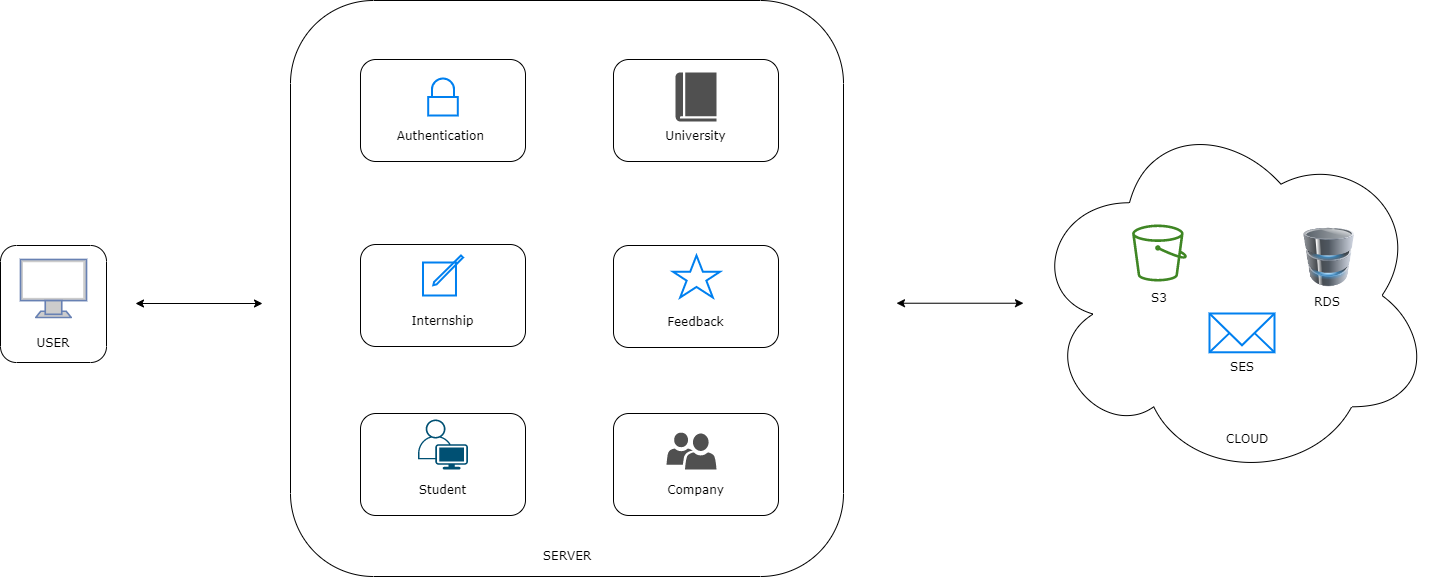
\includegraphics[scale=0.30]{Images/ImagesDD/overview.png}
    \caption{Overview diagram}
\end{figure}

The Students\&Companies (S\&C) platform is designed as a client-server application, where the term \textit{client} refers to the users of the system: students, companies, and universities. We have chosen a \textit{fat client} approach to provide a highly interactive, app-like experience, enabling responsive and rich functionality directly in the browser. This approach also reduces server load by offloading some processing to the client side, enhancing scalability.

Users interact with the system through a Single Page Application (SPA), a desktop web application that serves as the primary user interface for accessing platform features. The SPA allows for seamless navigation and interaction. By managing application state on the client side, the SPA minimizes page reloads, enhancing usability and responsiveness.

On the backend, we have followed a \textit{monolithic server} approach. This choice simplifies the overall system architecture by consolidating functionality into a single codebase, which can facilitate easier development, deployment, and maintenance. Although monolithic, the server is structured into multiple controllers and several business logic parts, each responsible for specific areas, such as authentication, internship management, profile handling, and recommendations. This modular organization within the monolith ensures that each component is cohesive and manageable while maintaining performance and consistency.

To support database, storage, and email services, we are using a cloud provider infrastructure. Specifically, we utilize Amazon Web Services (AWS) with Amazon RDS for the database, Amazon S3 for file storage, and Amazon SES for email notifications.


\newpage

\section{Component view}

\subsection{Client Components}
The principal component of the client side is the Web-App, which the user will interact with.

\subsection{Server Components}

In the server side, resides the principal components such as the controller used to manage the HTTP request sent by the user.

\begin{itemize}
\item \textbf{Internship}: Handles the logic related to managing internships, including creating, updating, and tracking internship opportunities. It allows administrators and companies to post internship positions and lets students apply, track, and view their application statuses.

\item \textbf{Student}: Manages all student-related data, including profile creation, academic details, and progress tracking. It allows students to update their profiles and view their application history, while administrators can monitor student progress and make updates as needed.

\item \textbf{Match}: Manages all the matches between the students and the companies' internship, finding matching between the suitable skills. Allows sending invitation to the student, and accepting those ones.

\item \textbf{Feedback}: Implements the system for collecting and managing feedback from students, companies, and administrators. This component allows participants to submit feedback on internship experiences, and administrators can review and analyze this feedback to improve the program.

\item \textbf{Company}: Responsible for managing company accounts and profiles, as well as facilitating company interactions with students and internships. It allows companies to create profiles, post internship opportunities, and review student applications, making the hiring and feedback process streamlined and accessible.

\item \textbf{University}: Responsible for managing university interaction with the platform. Such as tracking students' internship, reading their feedback and leaving a feedback about the platform.


\item \textbf{Authentication}:
The Authentication handles all processes related to user authentication, such as logging in, logging out, session validation, and password management.
\end{itemize}

\subsection{Data Component}

We use a relational database hosted on AWS to securely manage and organize structured data for the application. AWS’s managed RDS service offers high availability, automated backups, and scalability, ensuring reliable data storage and quick access for all server components. This setup allows us to maintain relational integrity, enforce data consistency, and easily scale as our data requirements grow.


\begin{figure}[!ht]
    \centering
    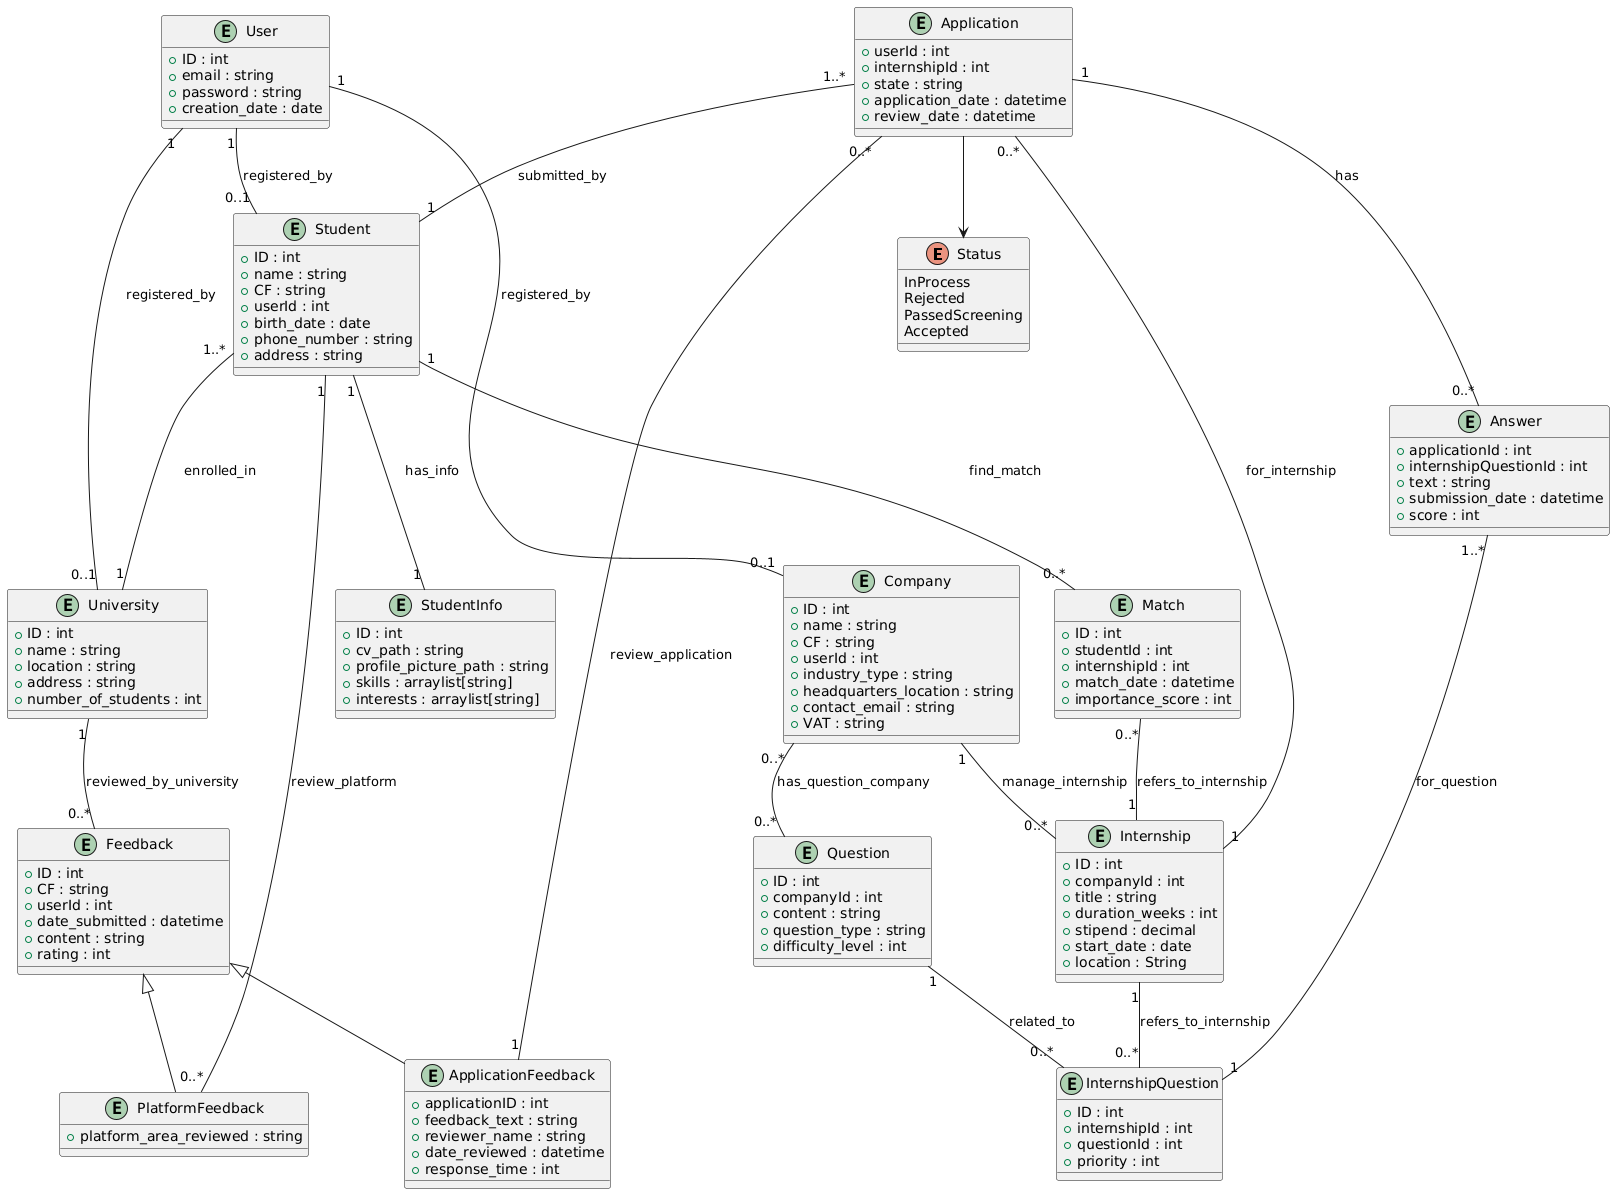
\includegraphics[scale=0.30]{Images/ImagesDD/class_diagram.png}
    \caption{Class diagram referring to the data components}
\end{figure}


\section{Deployment view}

The frontend is a SPA implemented with the React framework. The website can be visited from any modern web browser, such as Google Chrome, Mozilla Firefox or Microsoft Edge. \\ \\
Clients can be any desktop device that can run the previous browsers, such as computers with Windows, Linux or macOS.
The website is served by a CDN like Amazon CloudFront.
Using a CDN greatly enhances performance by caching static assets on globally distributed servers, ensuring users access content from locations closest to them for faster load times and reduced latency. \\ \\
The backend of the platform is powered by an ASP.NET Core server, deployed within a Kubernetes cluster that orchestrates and manages the containerized environment. This setup ensures that the backend is scalable, resilient, and highly available, with Kubernetes automating the deployment, scaling, and management of application pods. NGINX is used within the cluster as an Ingress Controller, handling incoming traffic, SSL termination, and advanced routing rules. Kubernetes performs horizontal scaling by automatically deploying new pods during traffic surges to maintain seamless performance.\\ \\
The ASP.NET Core application communicates with AWS services like RDS for database and S3 for storage. Continuous integration and deployment pipelines facilitate automated updates, pushing new Docker images to the cluster and enabling rolling updates with minimal downtime.\\ \\
This integration of Kubernetes and NGINX ensures that the backend infrastructure is robust and adaptable, capable of handling large volumes of requests while providing efficient load distribution and reliability.

\begin{figure}[!ht]
    \centering
    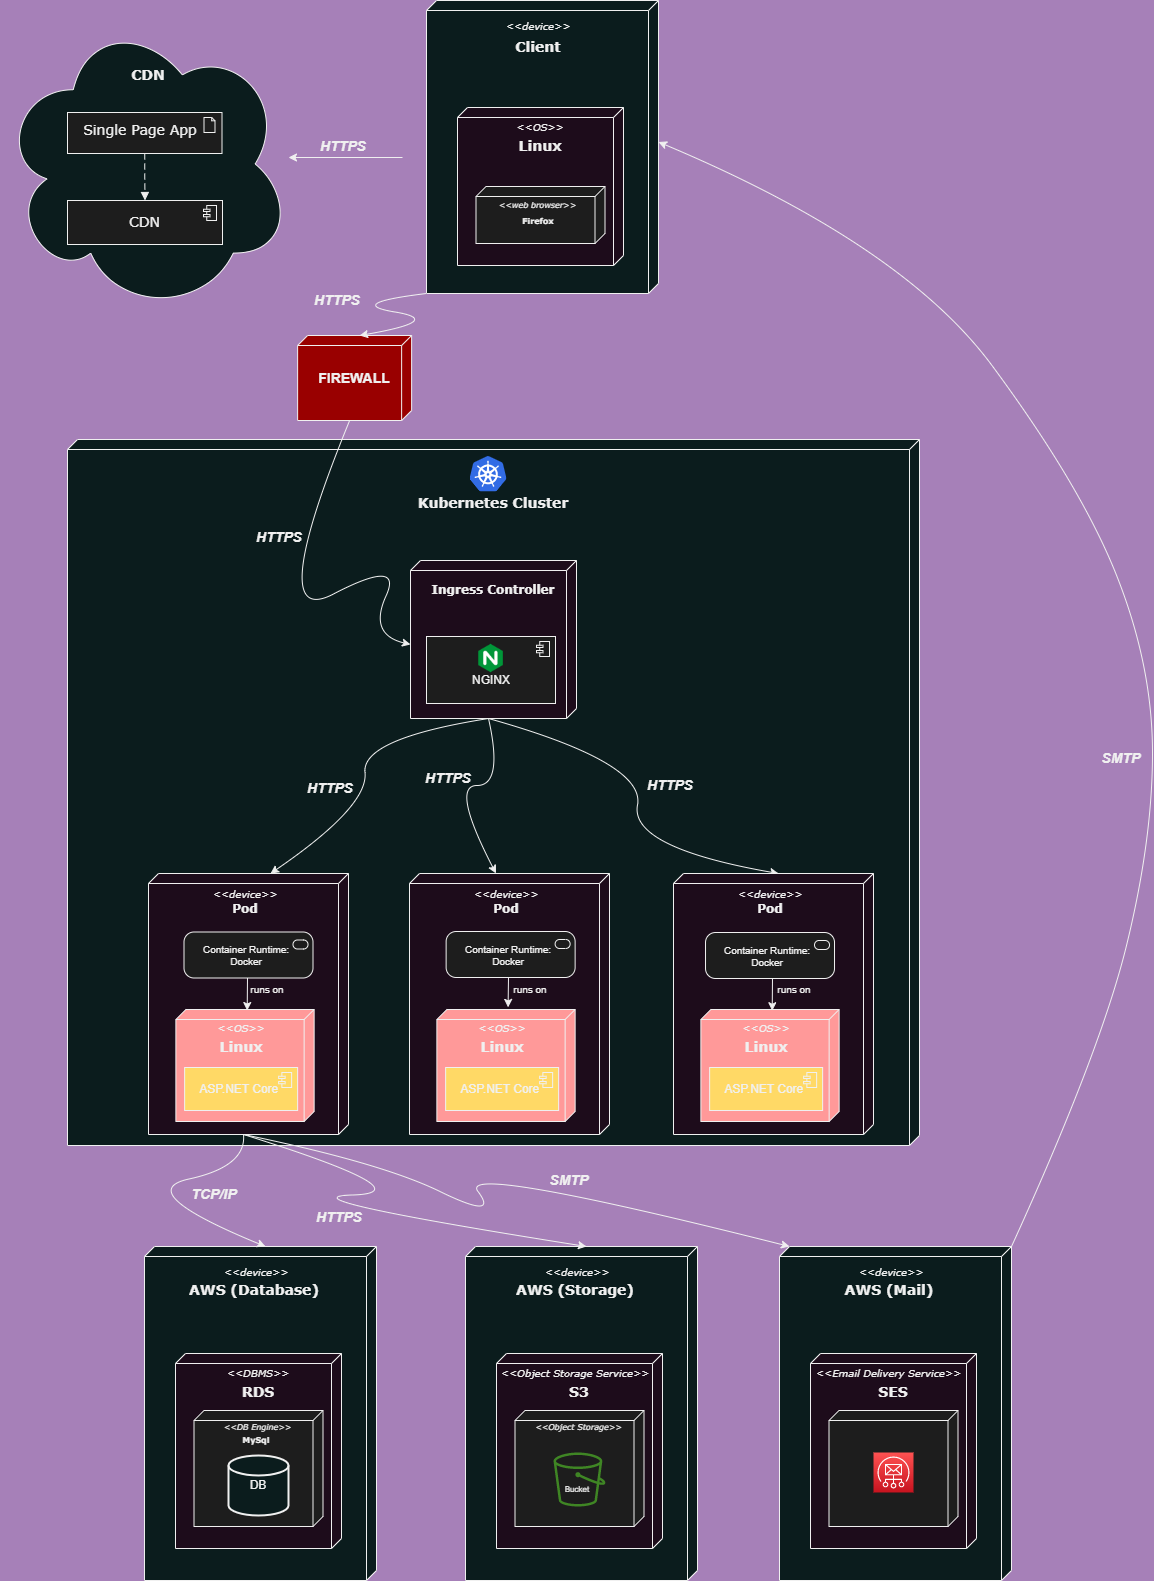
\includegraphics[scale=0.30]{Images/ImagesDD/deployment.png}
    \caption{Deployment diagram}
\end{figure}

\newpage


\section{Runtime view}
The following sequence diagrams illustrate the interactions between system components. 

Each diagram corresponds to and represents the implementation of its respective use case, as described in the RASD document, in the same order.

In each sequence diagram it is omitted the part specified in the diagram 0.1, that illustrates the case of unauthorized access and the tentative to gain a new valid authentication token. 

The following function (2.2) for simplicity is represented in another diagram, but it is meant to be intended as an action that happens before all the other diagrams.
\vspace{5mm}

\begin{figure}[ht!]
    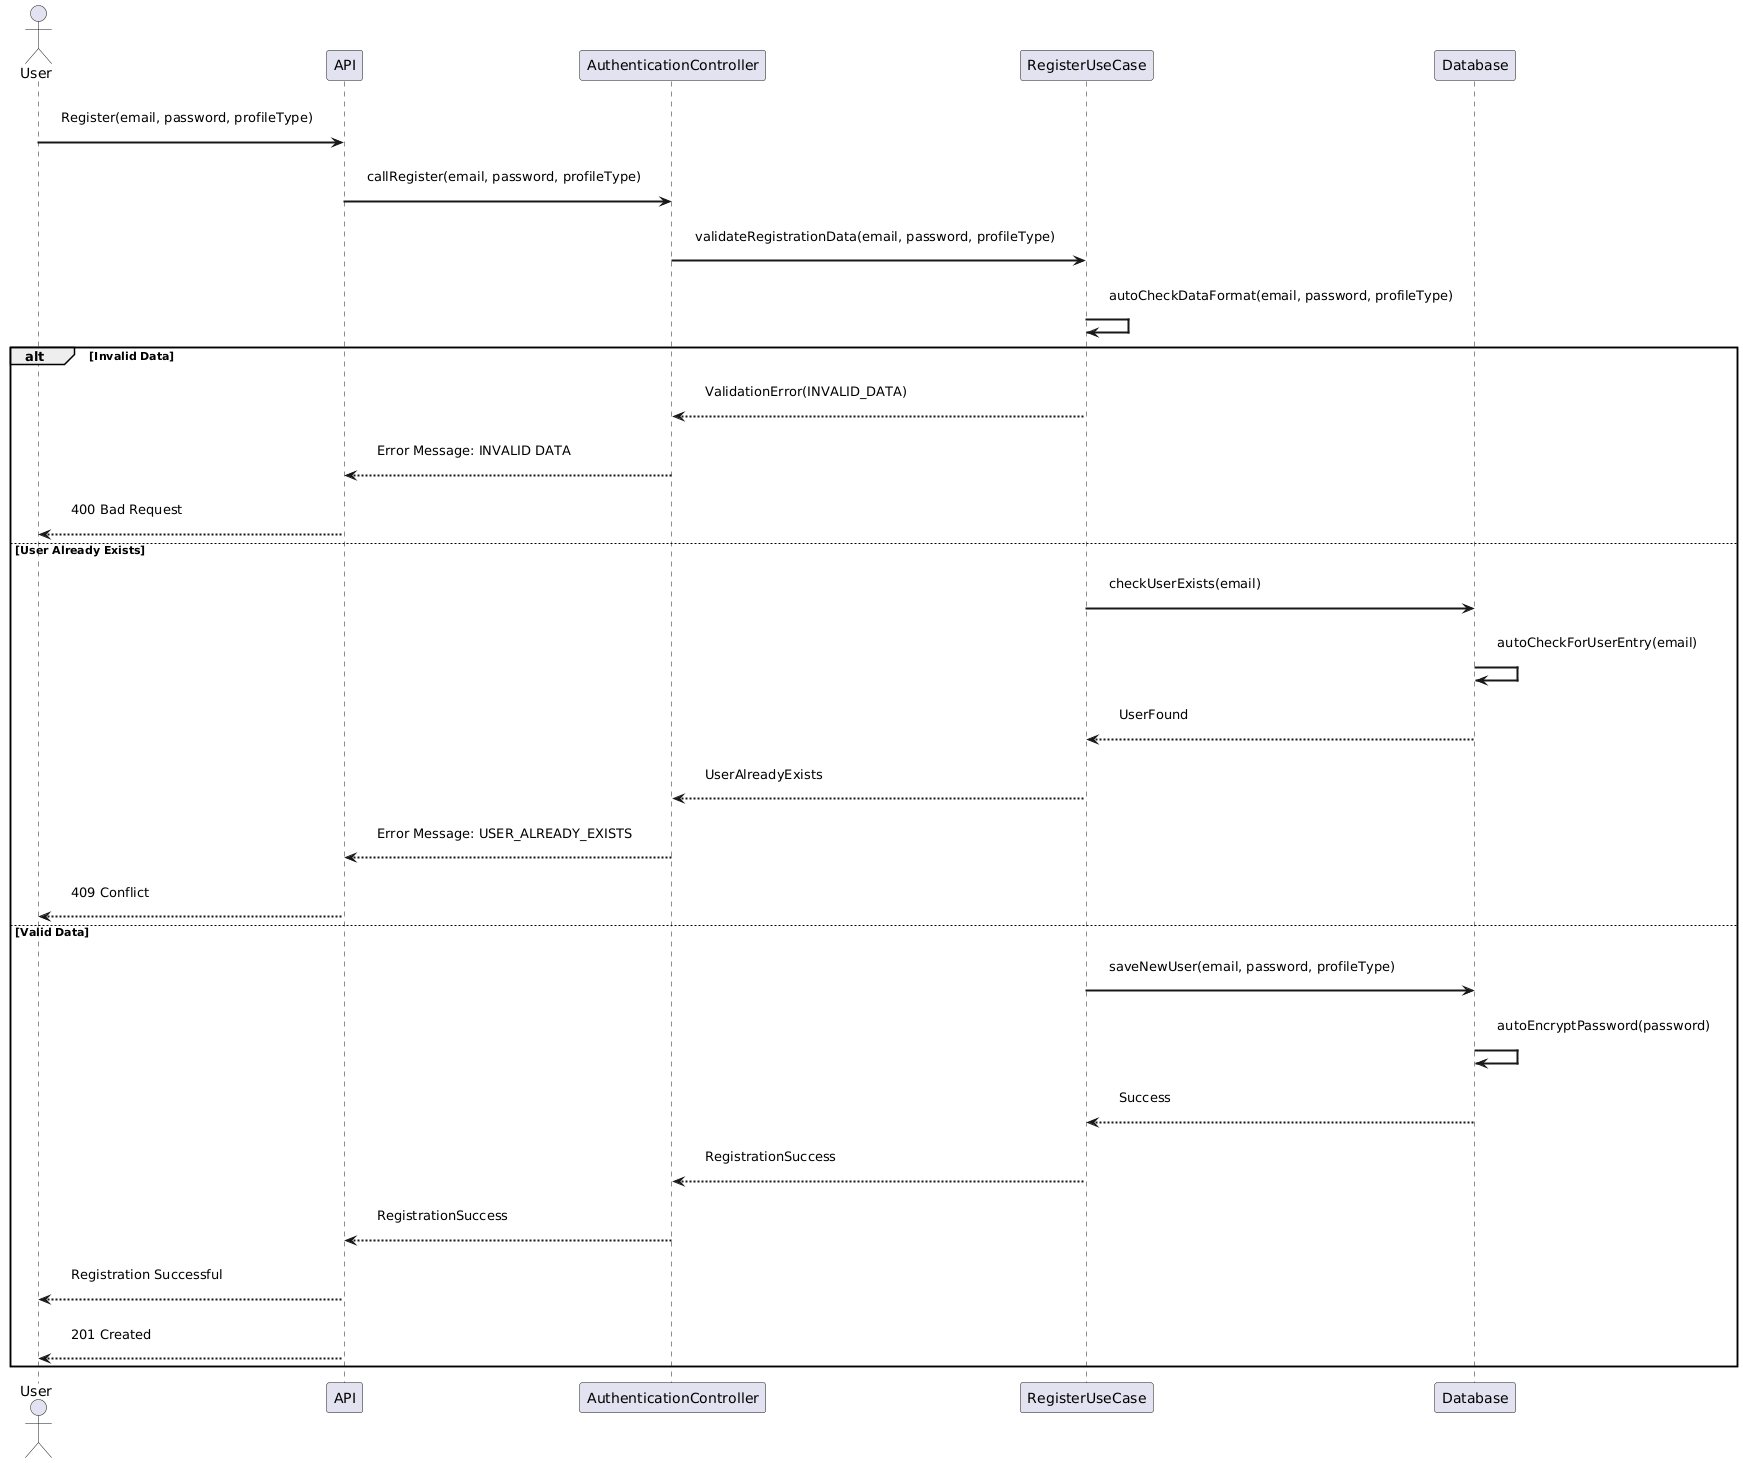
\includegraphics[scale=0.29]{Images/ImagesSequenceDiagram/RegisterAuthentication.png}
    \caption{User (Student, Company or University) Registration}
\end{figure}

\newpage

\begin{figure}[ht!]
    \centering
    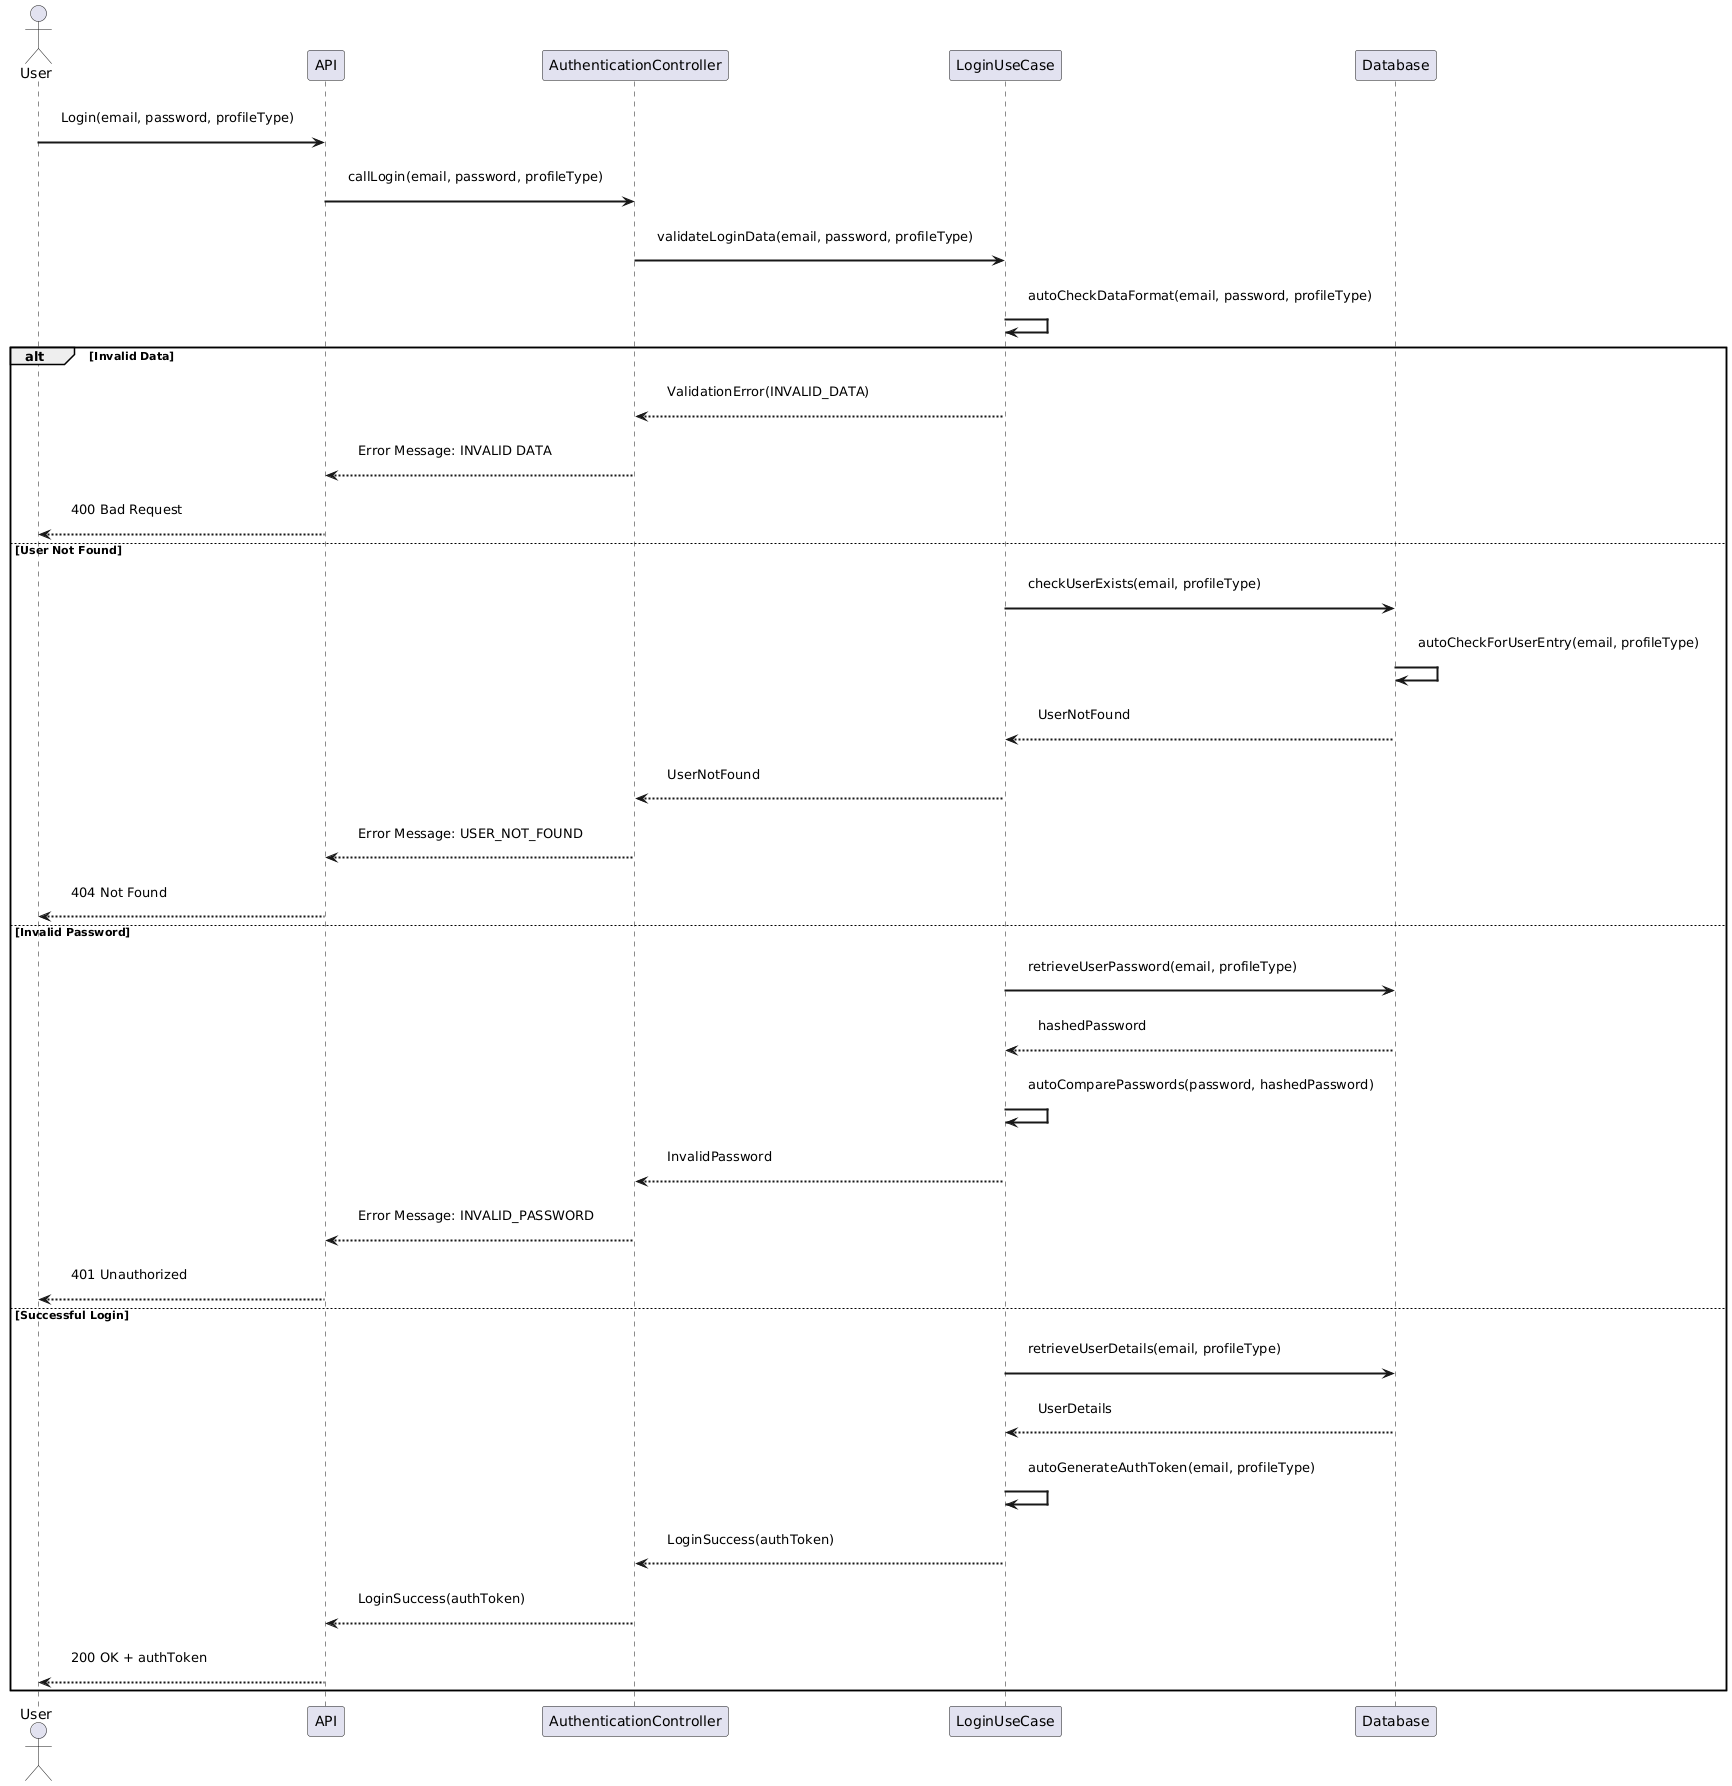
\includegraphics[scale=0.27]{Images/ImagesSequenceDiagram/LoginAuthentication.png}
    \caption{User (Student, Company or University) Login}
\end{figure}

\newpage

\begin{figure}[ht!]
    \centering
    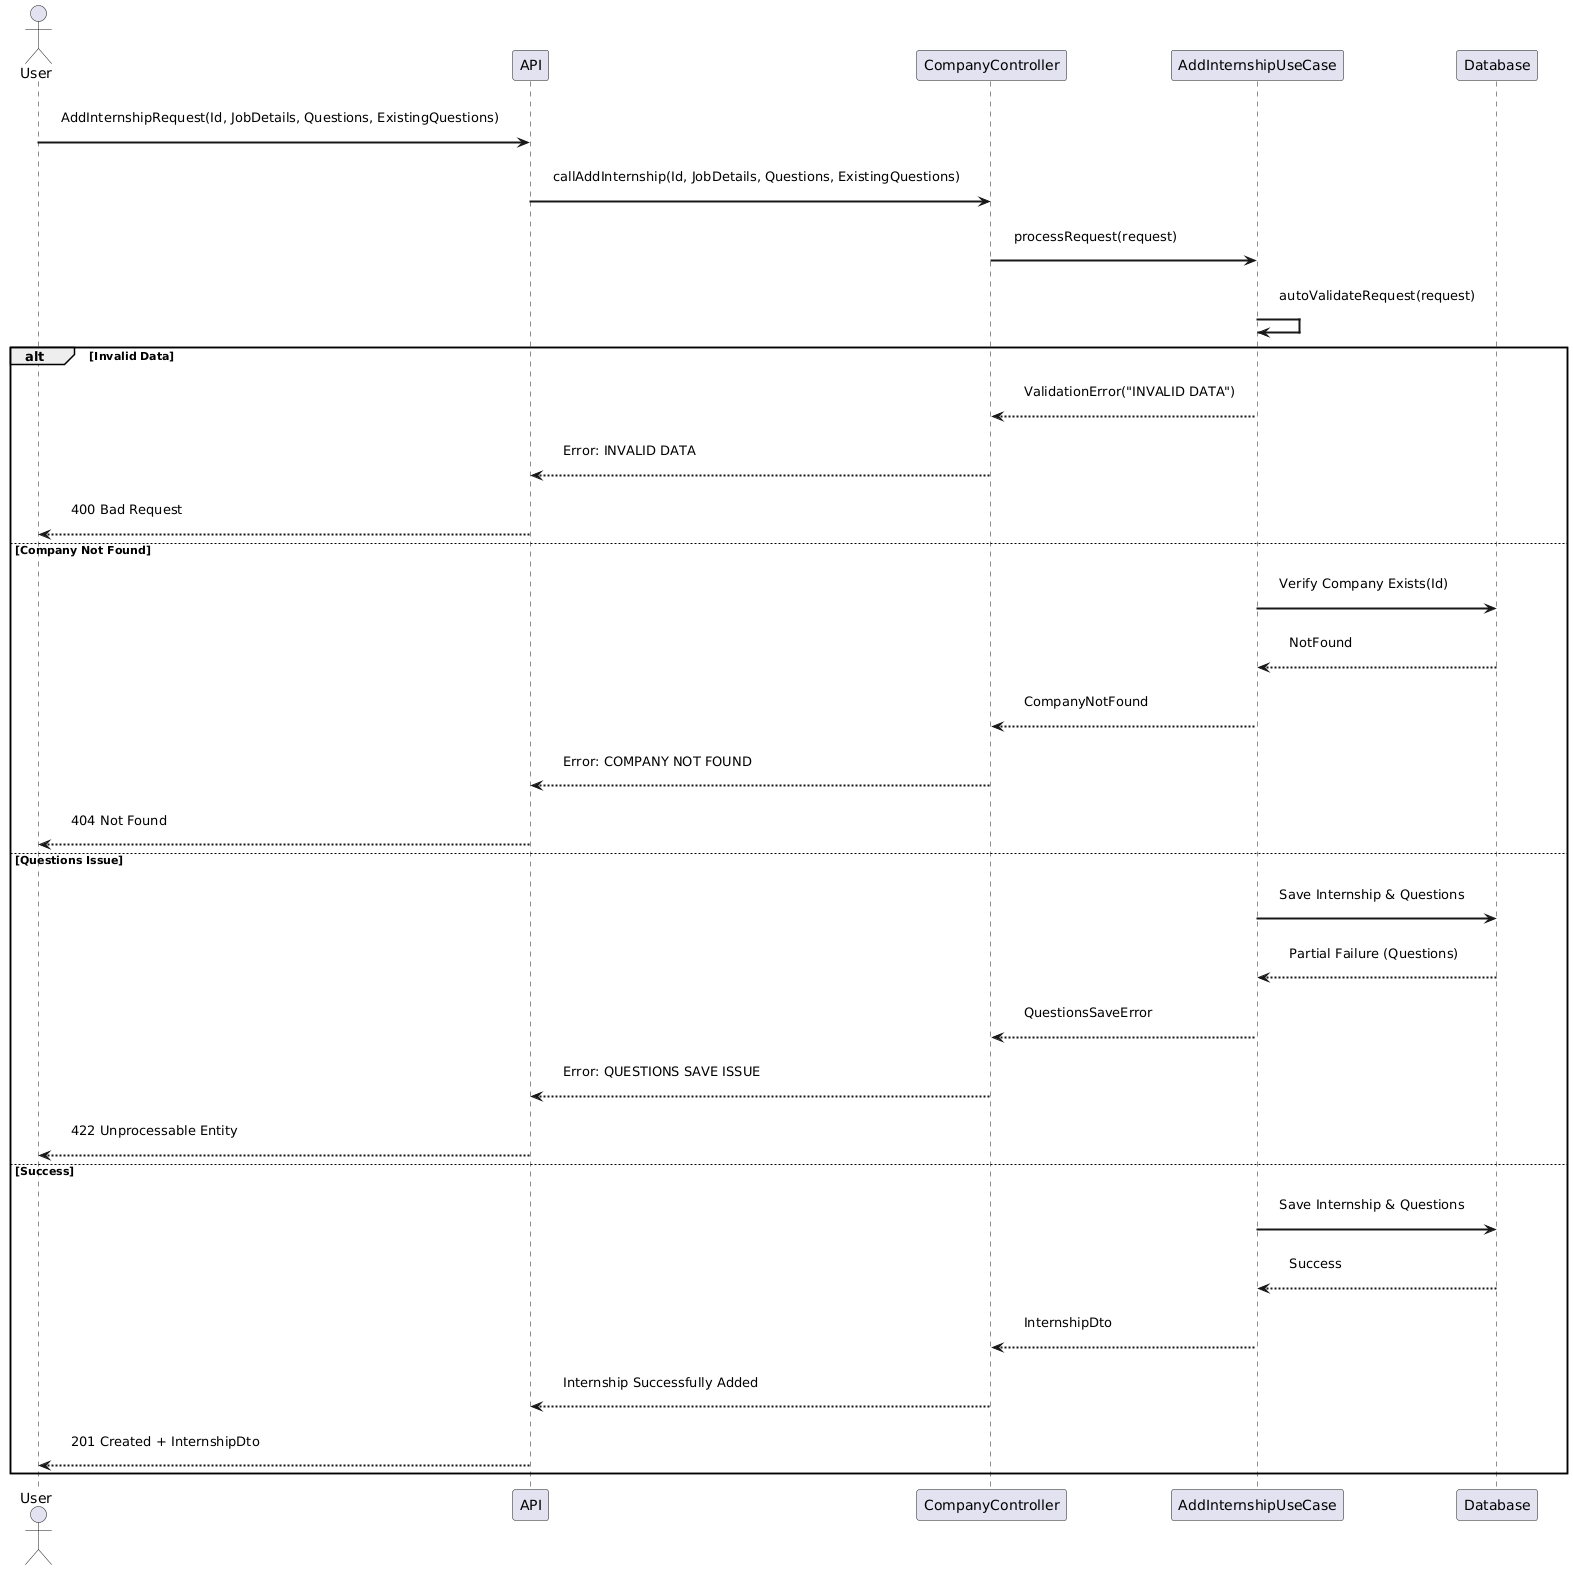
\includegraphics[scale=0.3]{Images/ImagesSequenceDiagram/InternshipCreation.png}
    \caption{Internship post creation}
\end{figure}

\newpage

\begin{figure}[ht!]
    \centering
    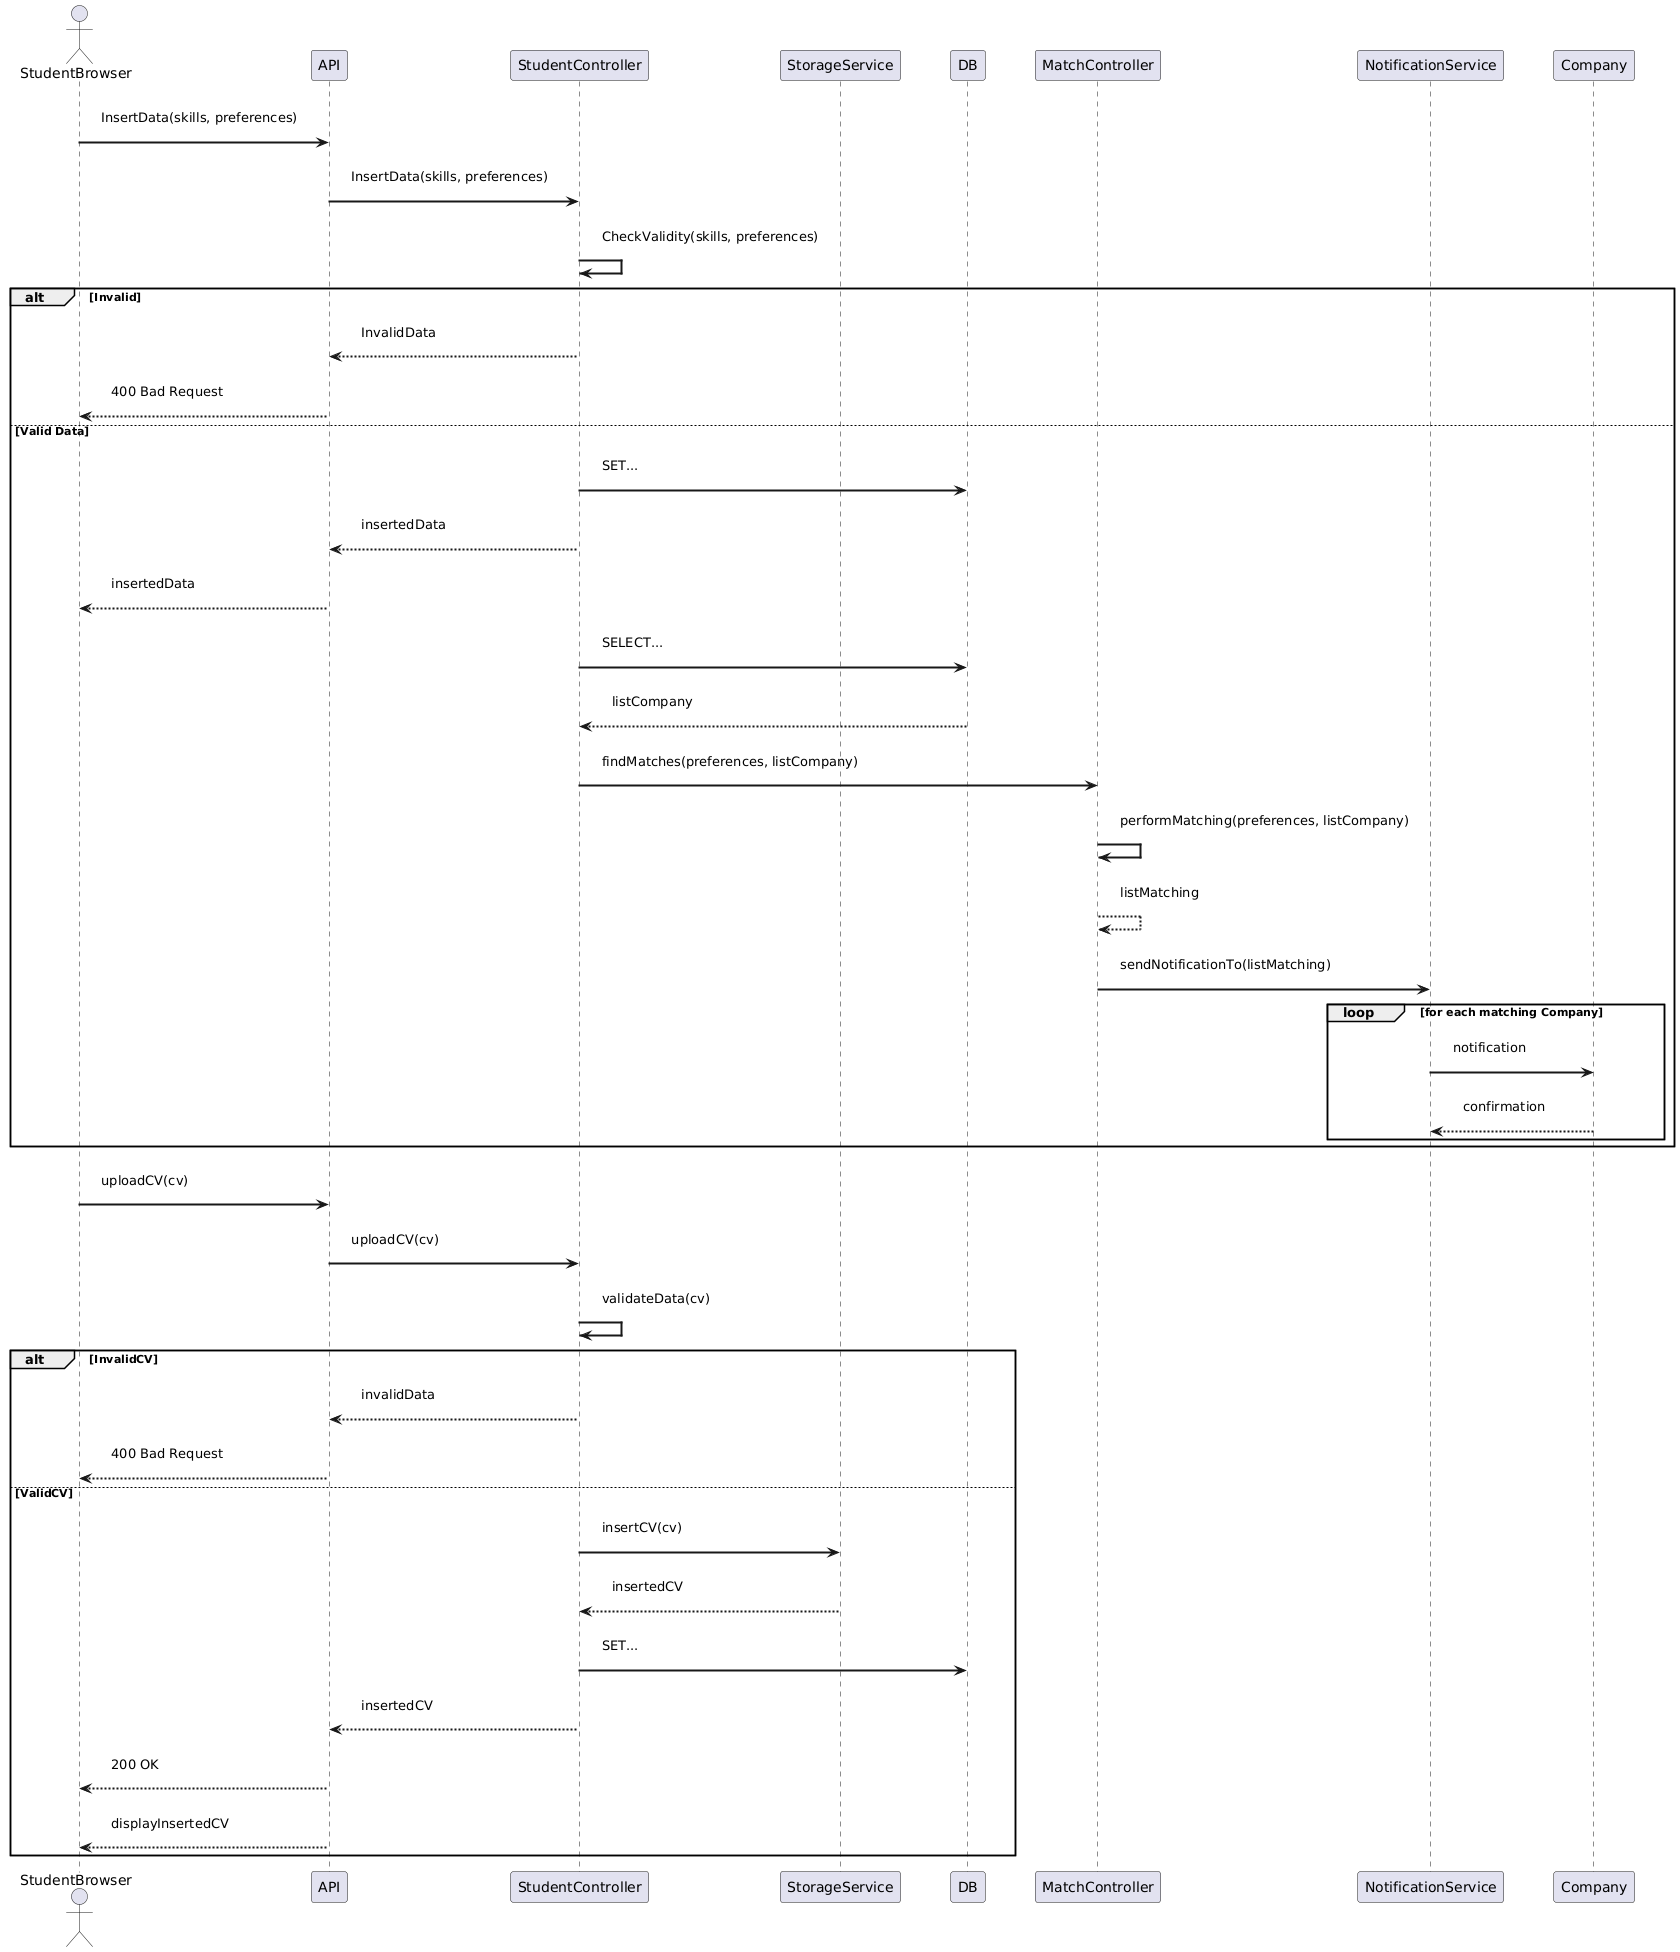
\includegraphics[scale=0.28]{Images/ImagesSequenceDiagram/StudentUploadCV.png}
    \caption{Student inserts CV and data}
\end{figure}

\newpage

\begin{figure}[ht!]
    \centering
    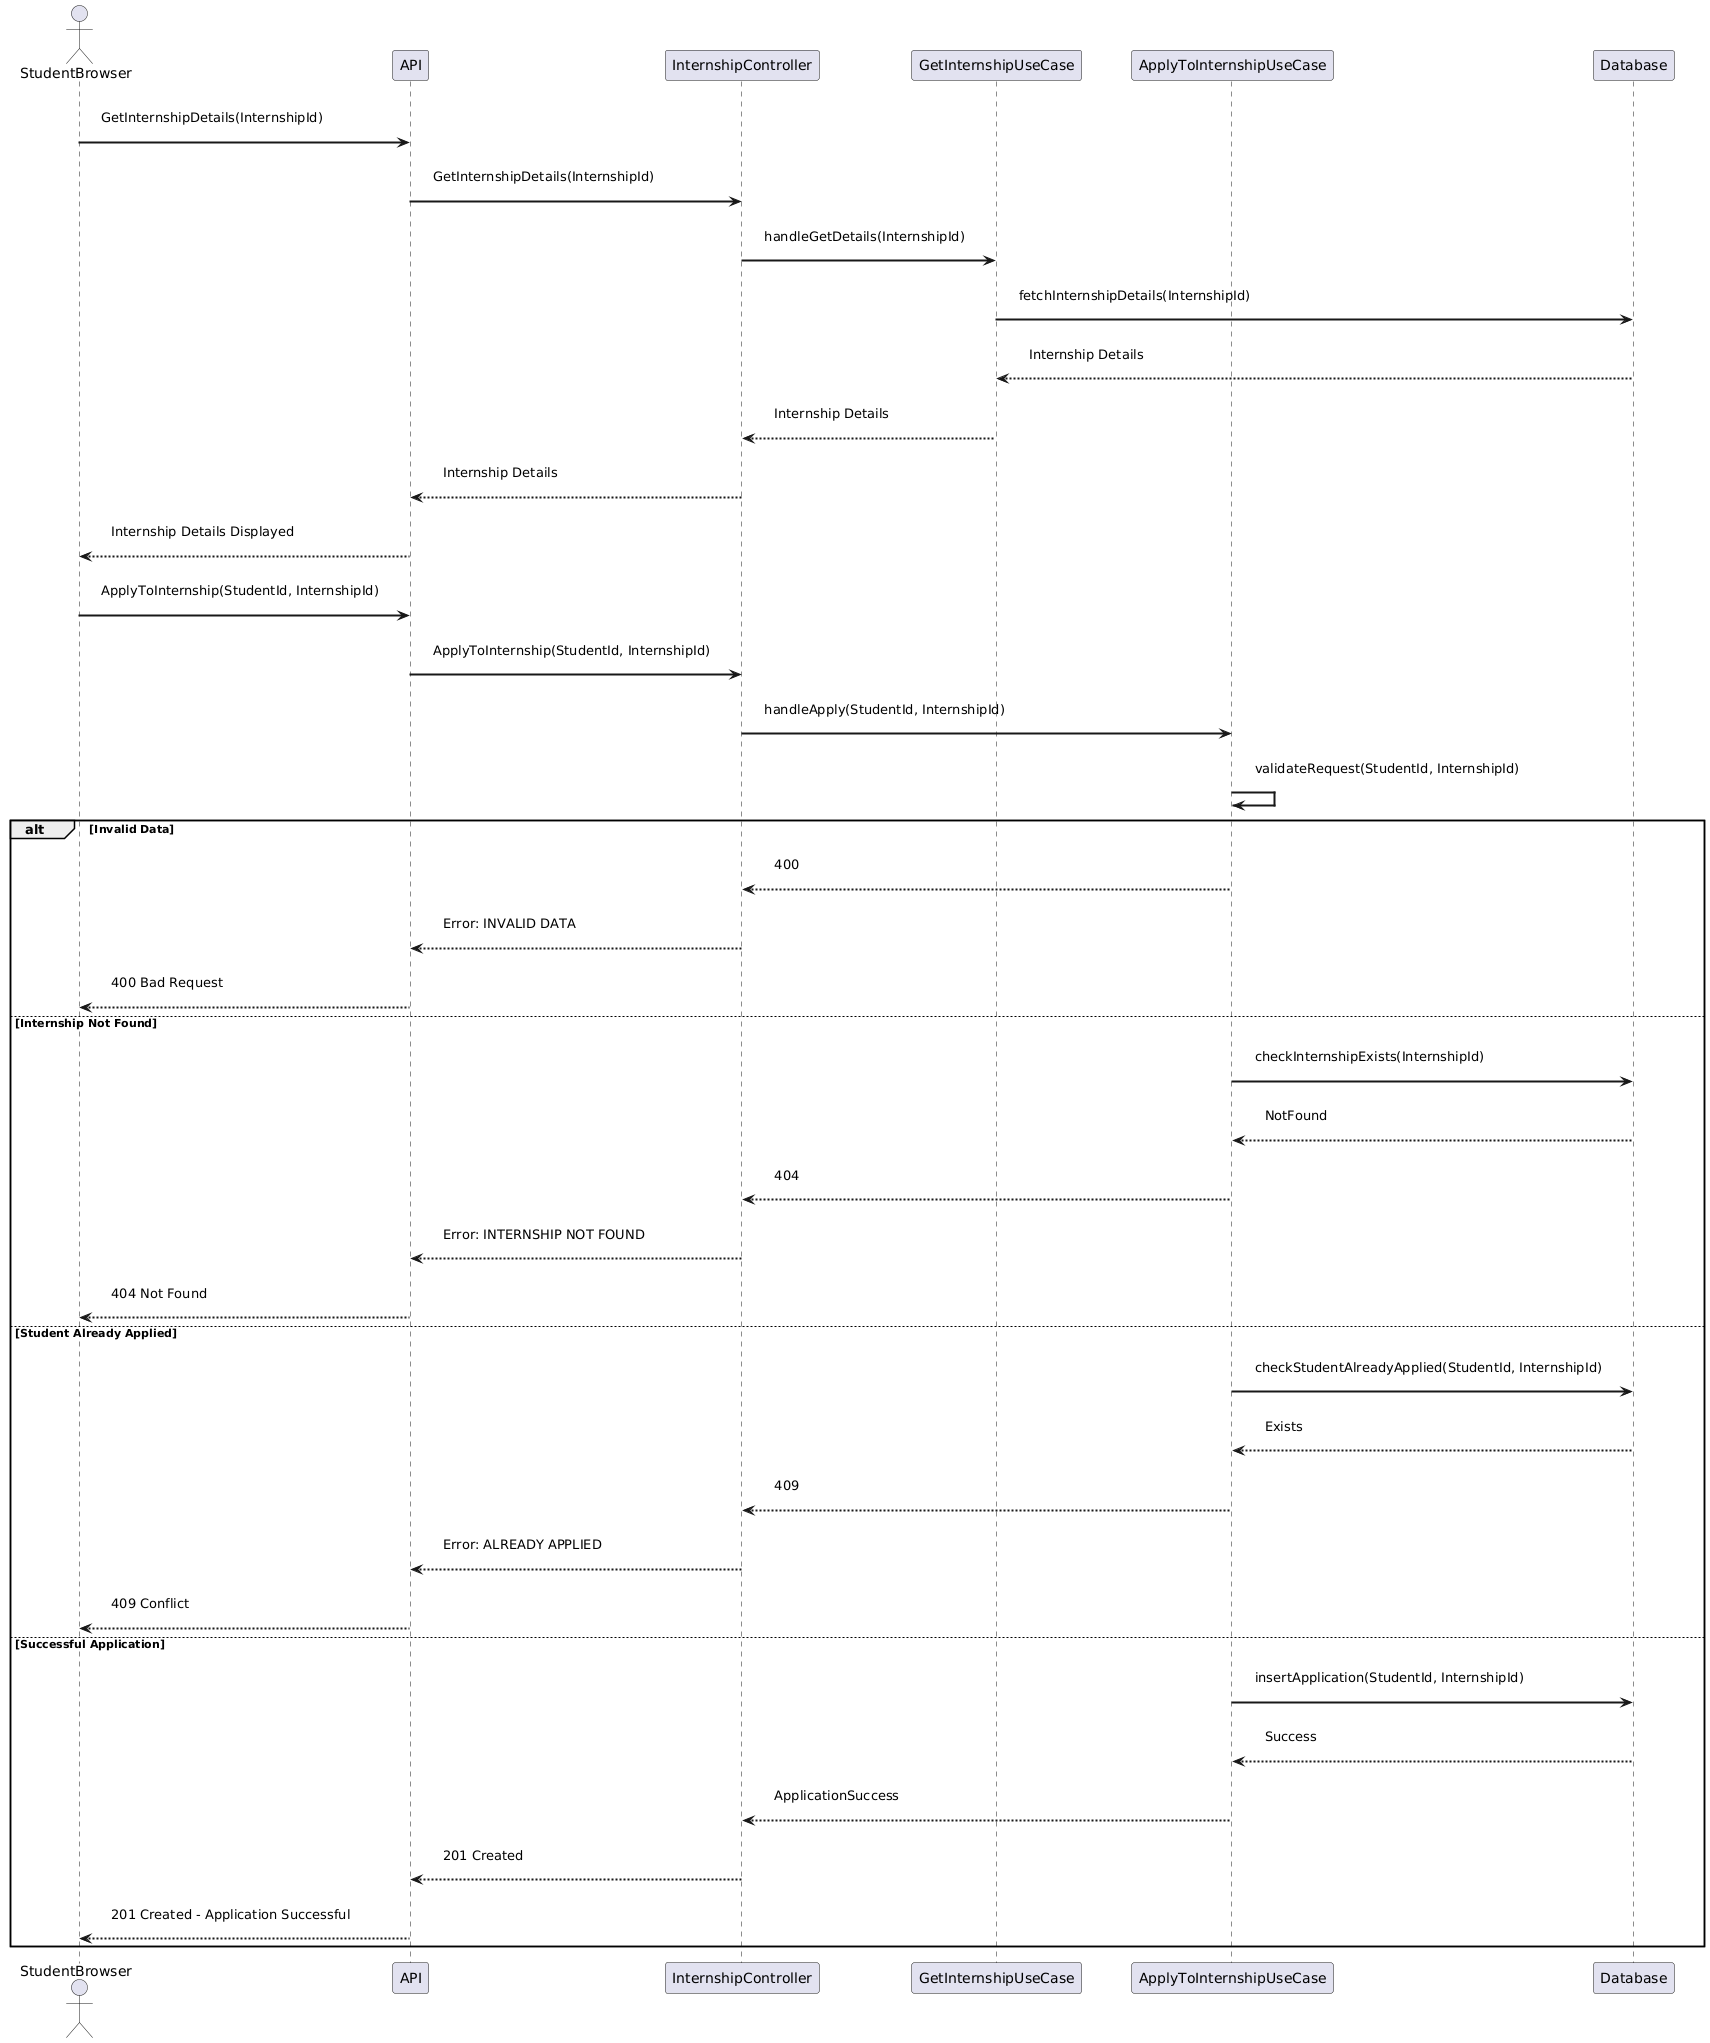
\includegraphics[scale=0.28]{Images/ImagesSequenceDiagram/StudentSubmitApplication.png}
    \caption{Student submit an application to an internship}
\end{figure}

\newpage

\begin{figure}[ht!]
    \centering
    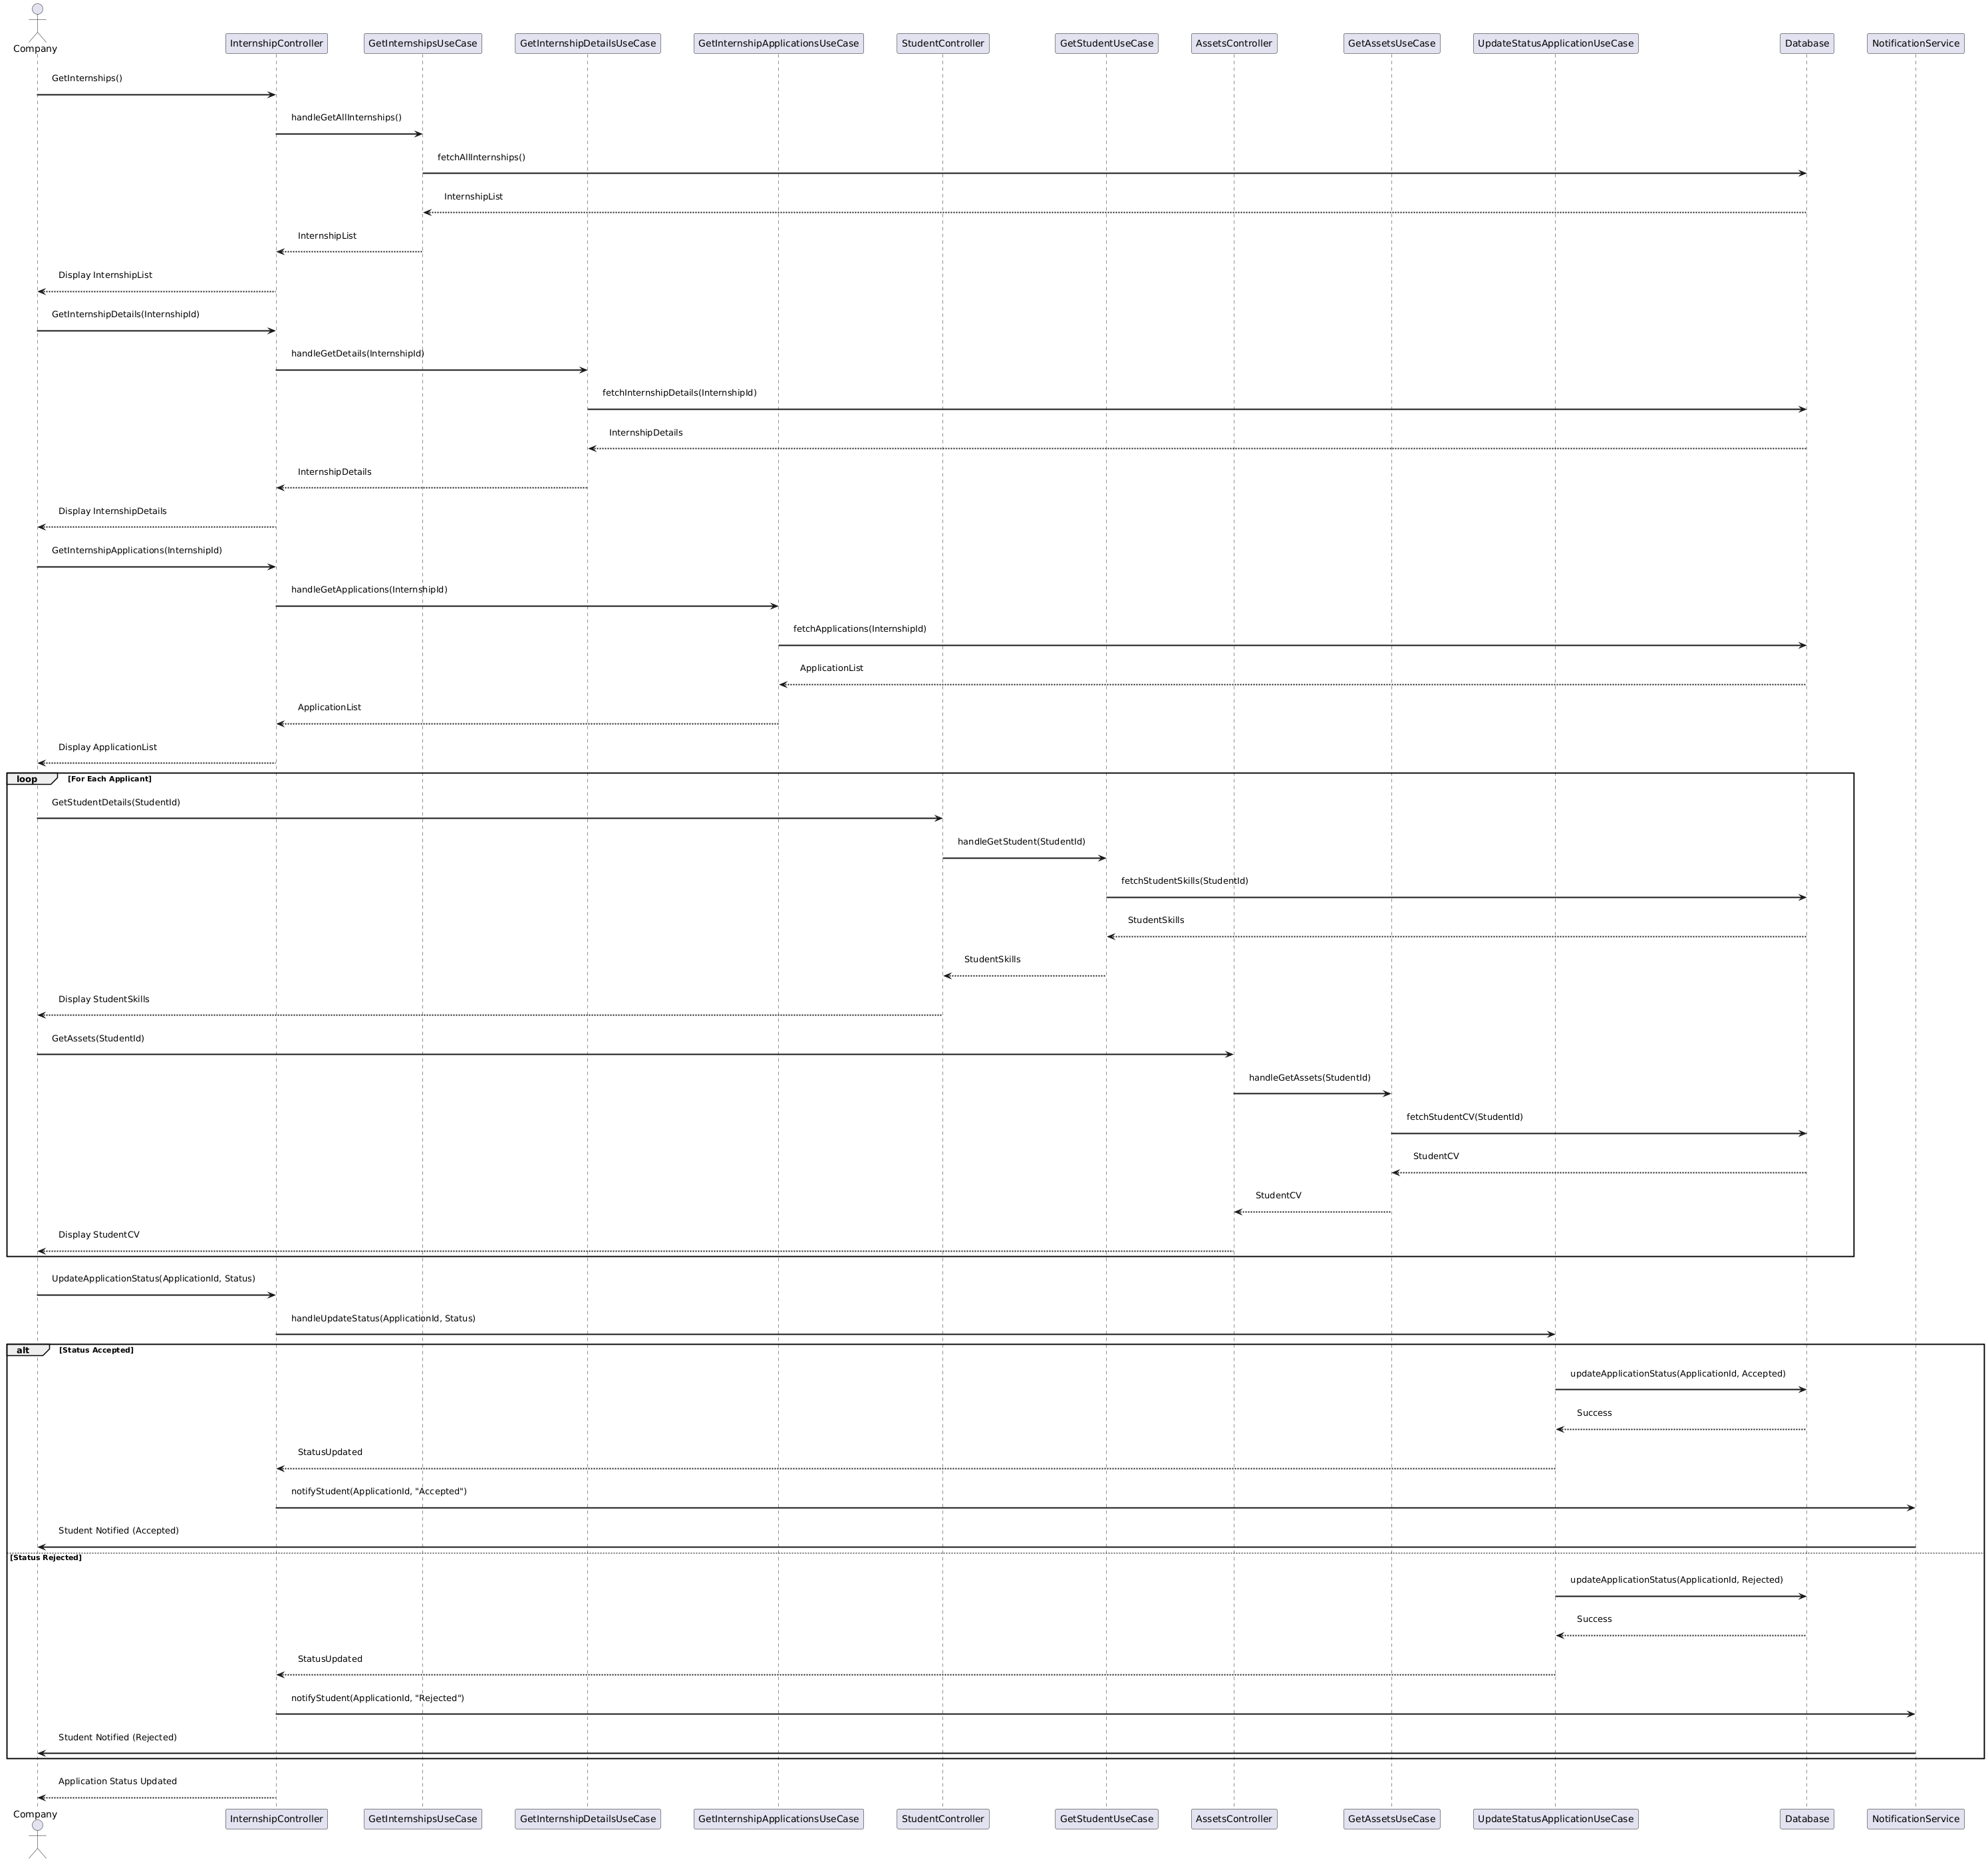
\includegraphics[scale=0.15]{Images/ImagesSequenceDiagram/CompanyManagesIncomeApplications.png}
    \caption{Company management of internship applications}
\end{figure}

\newpage

\begin{figure}[ht!]
    \centering
    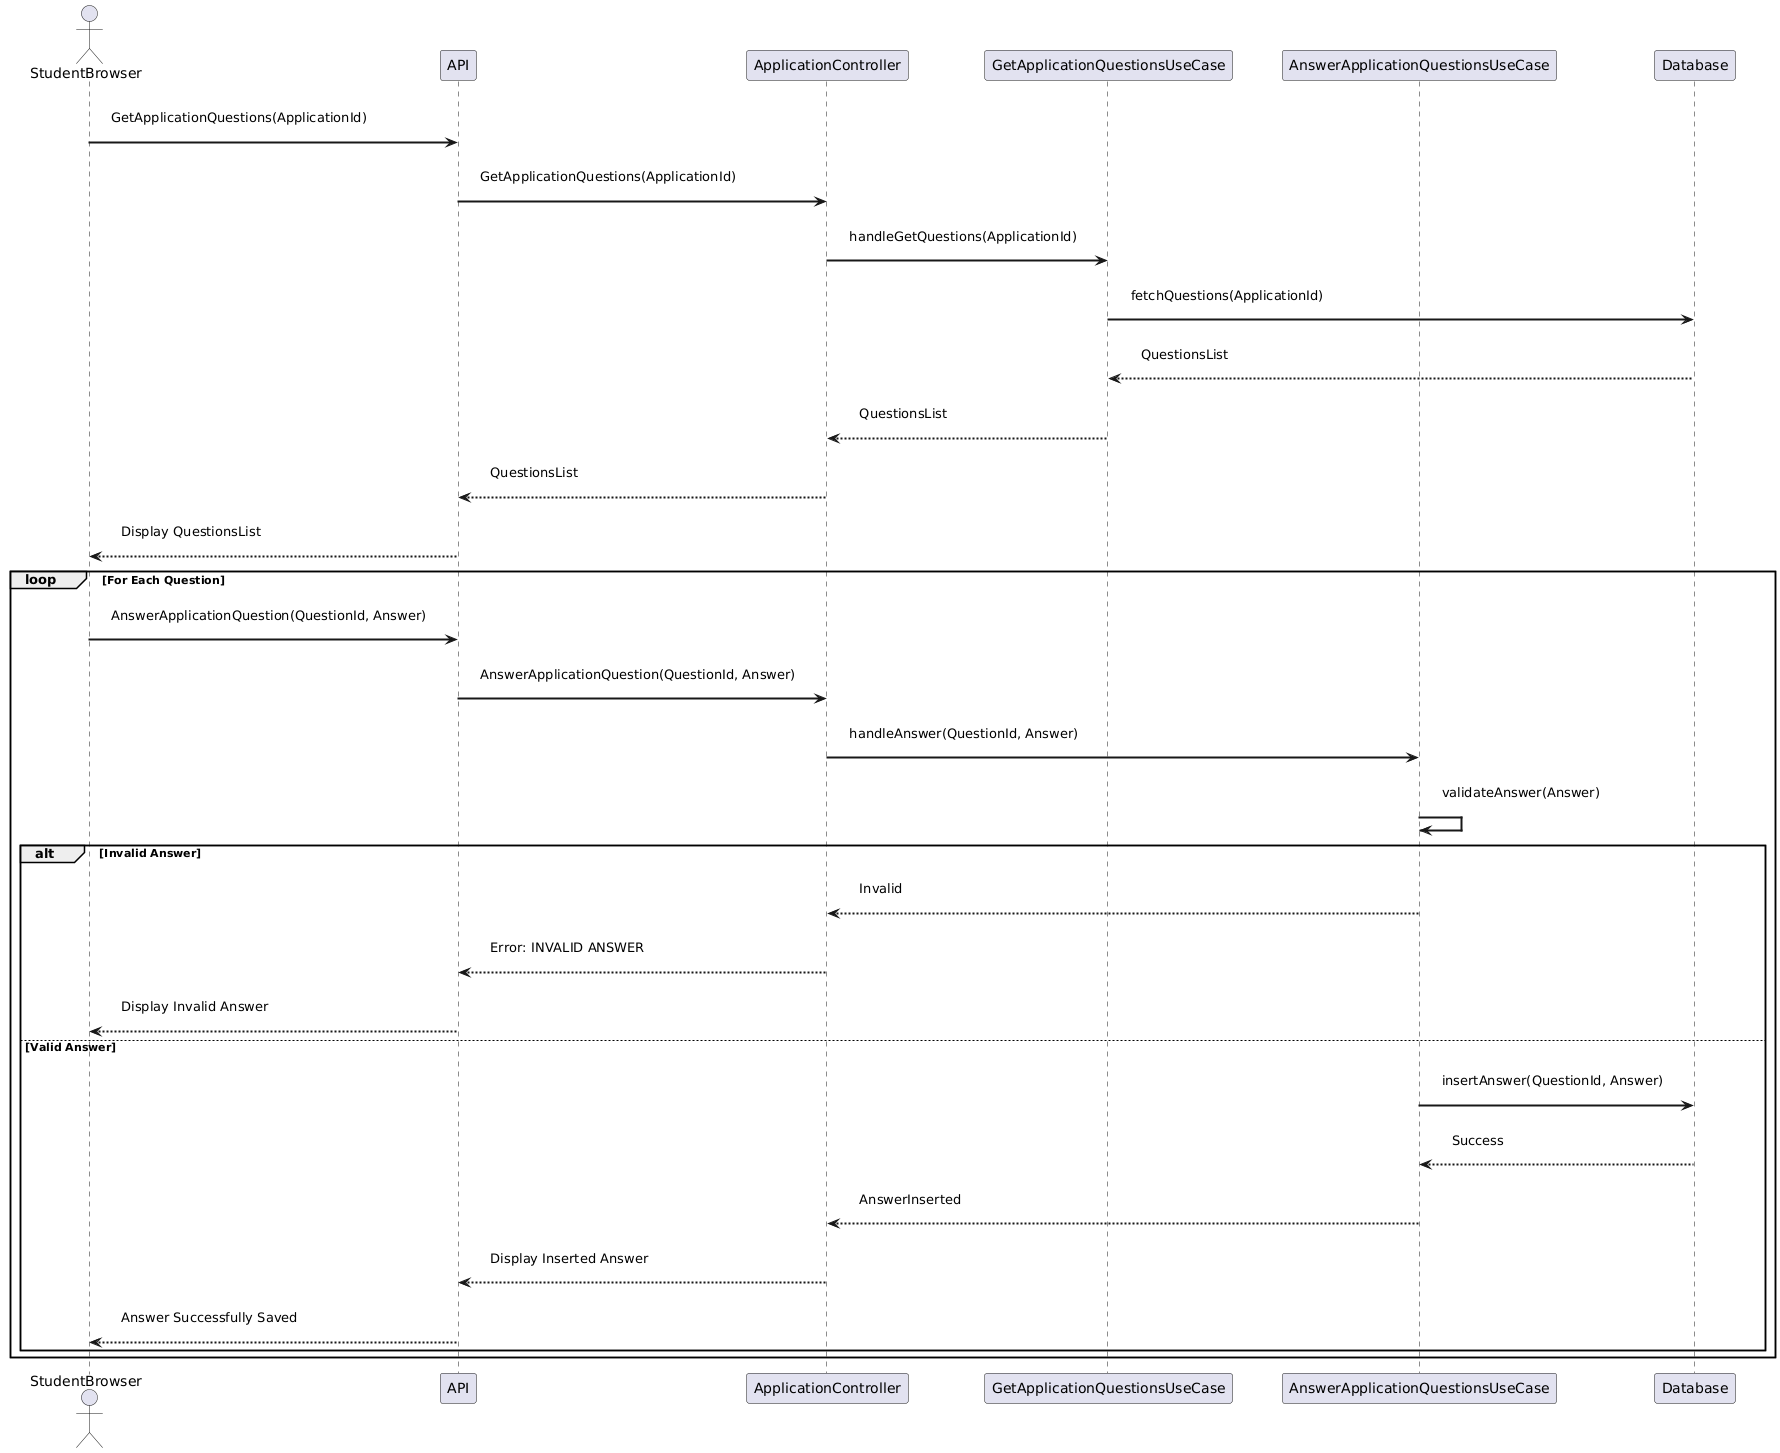
\includegraphics[scale=0.28]{Images/ImagesSequenceDiagram/StudentAnswereQuestions.png}
    \caption{Student answers questions}
\end{figure}

\newpage

\begin{figure}[ht!]
    \centering
    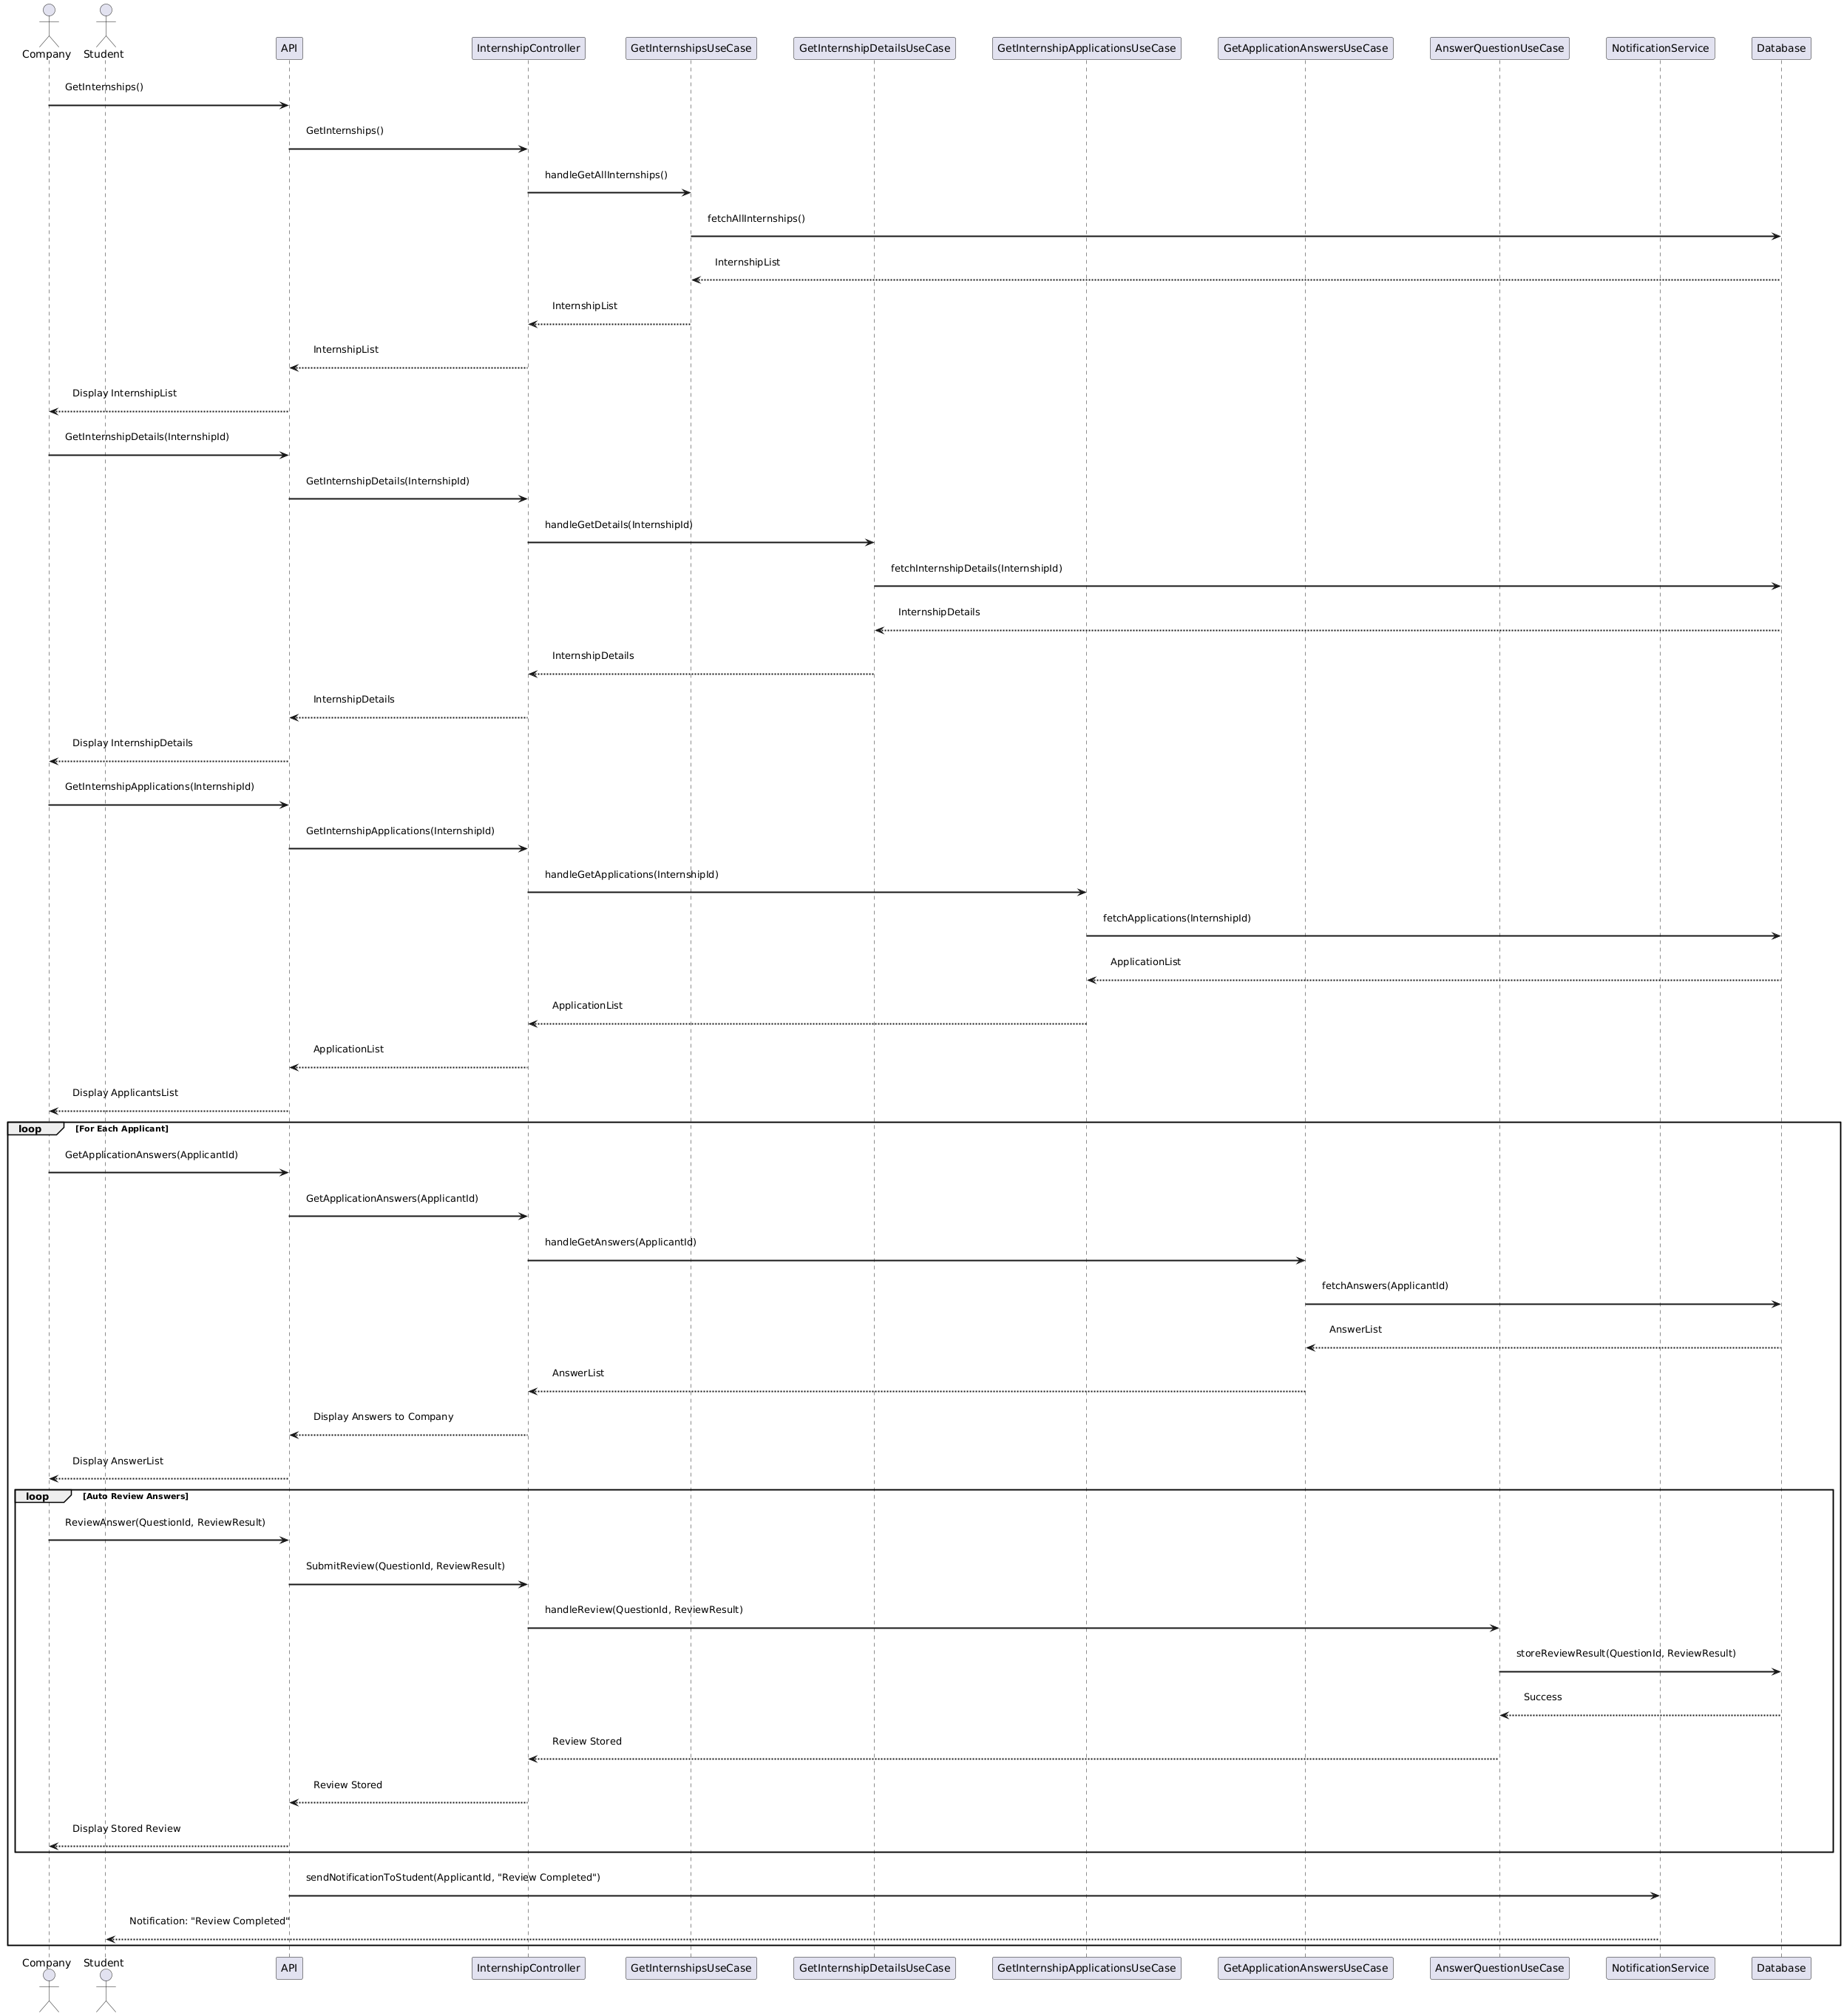
\includegraphics[scale=0.19]{Images/ImagesSequenceDiagram/CompanyReviewsQuestions.png}
    \caption{Company reviews online assessment questions}
\end{figure}

\newpage

\begin{figure}[ht!]
    \centering
    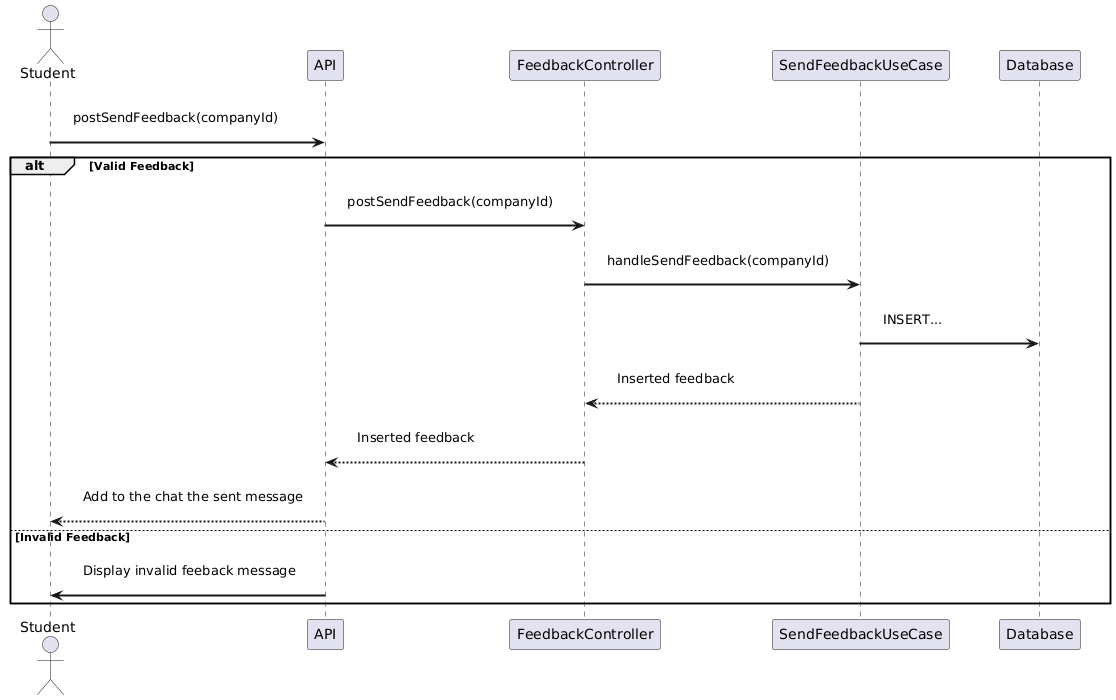
\includegraphics[scale=0.4]{Images/ImagesSequenceDiagram/SendFeebackSD.png}
    \caption{Student(Company) sends feedback to the platform.}
\end{figure}


\newpage

\begin{figure}[ht!]
    \centering
    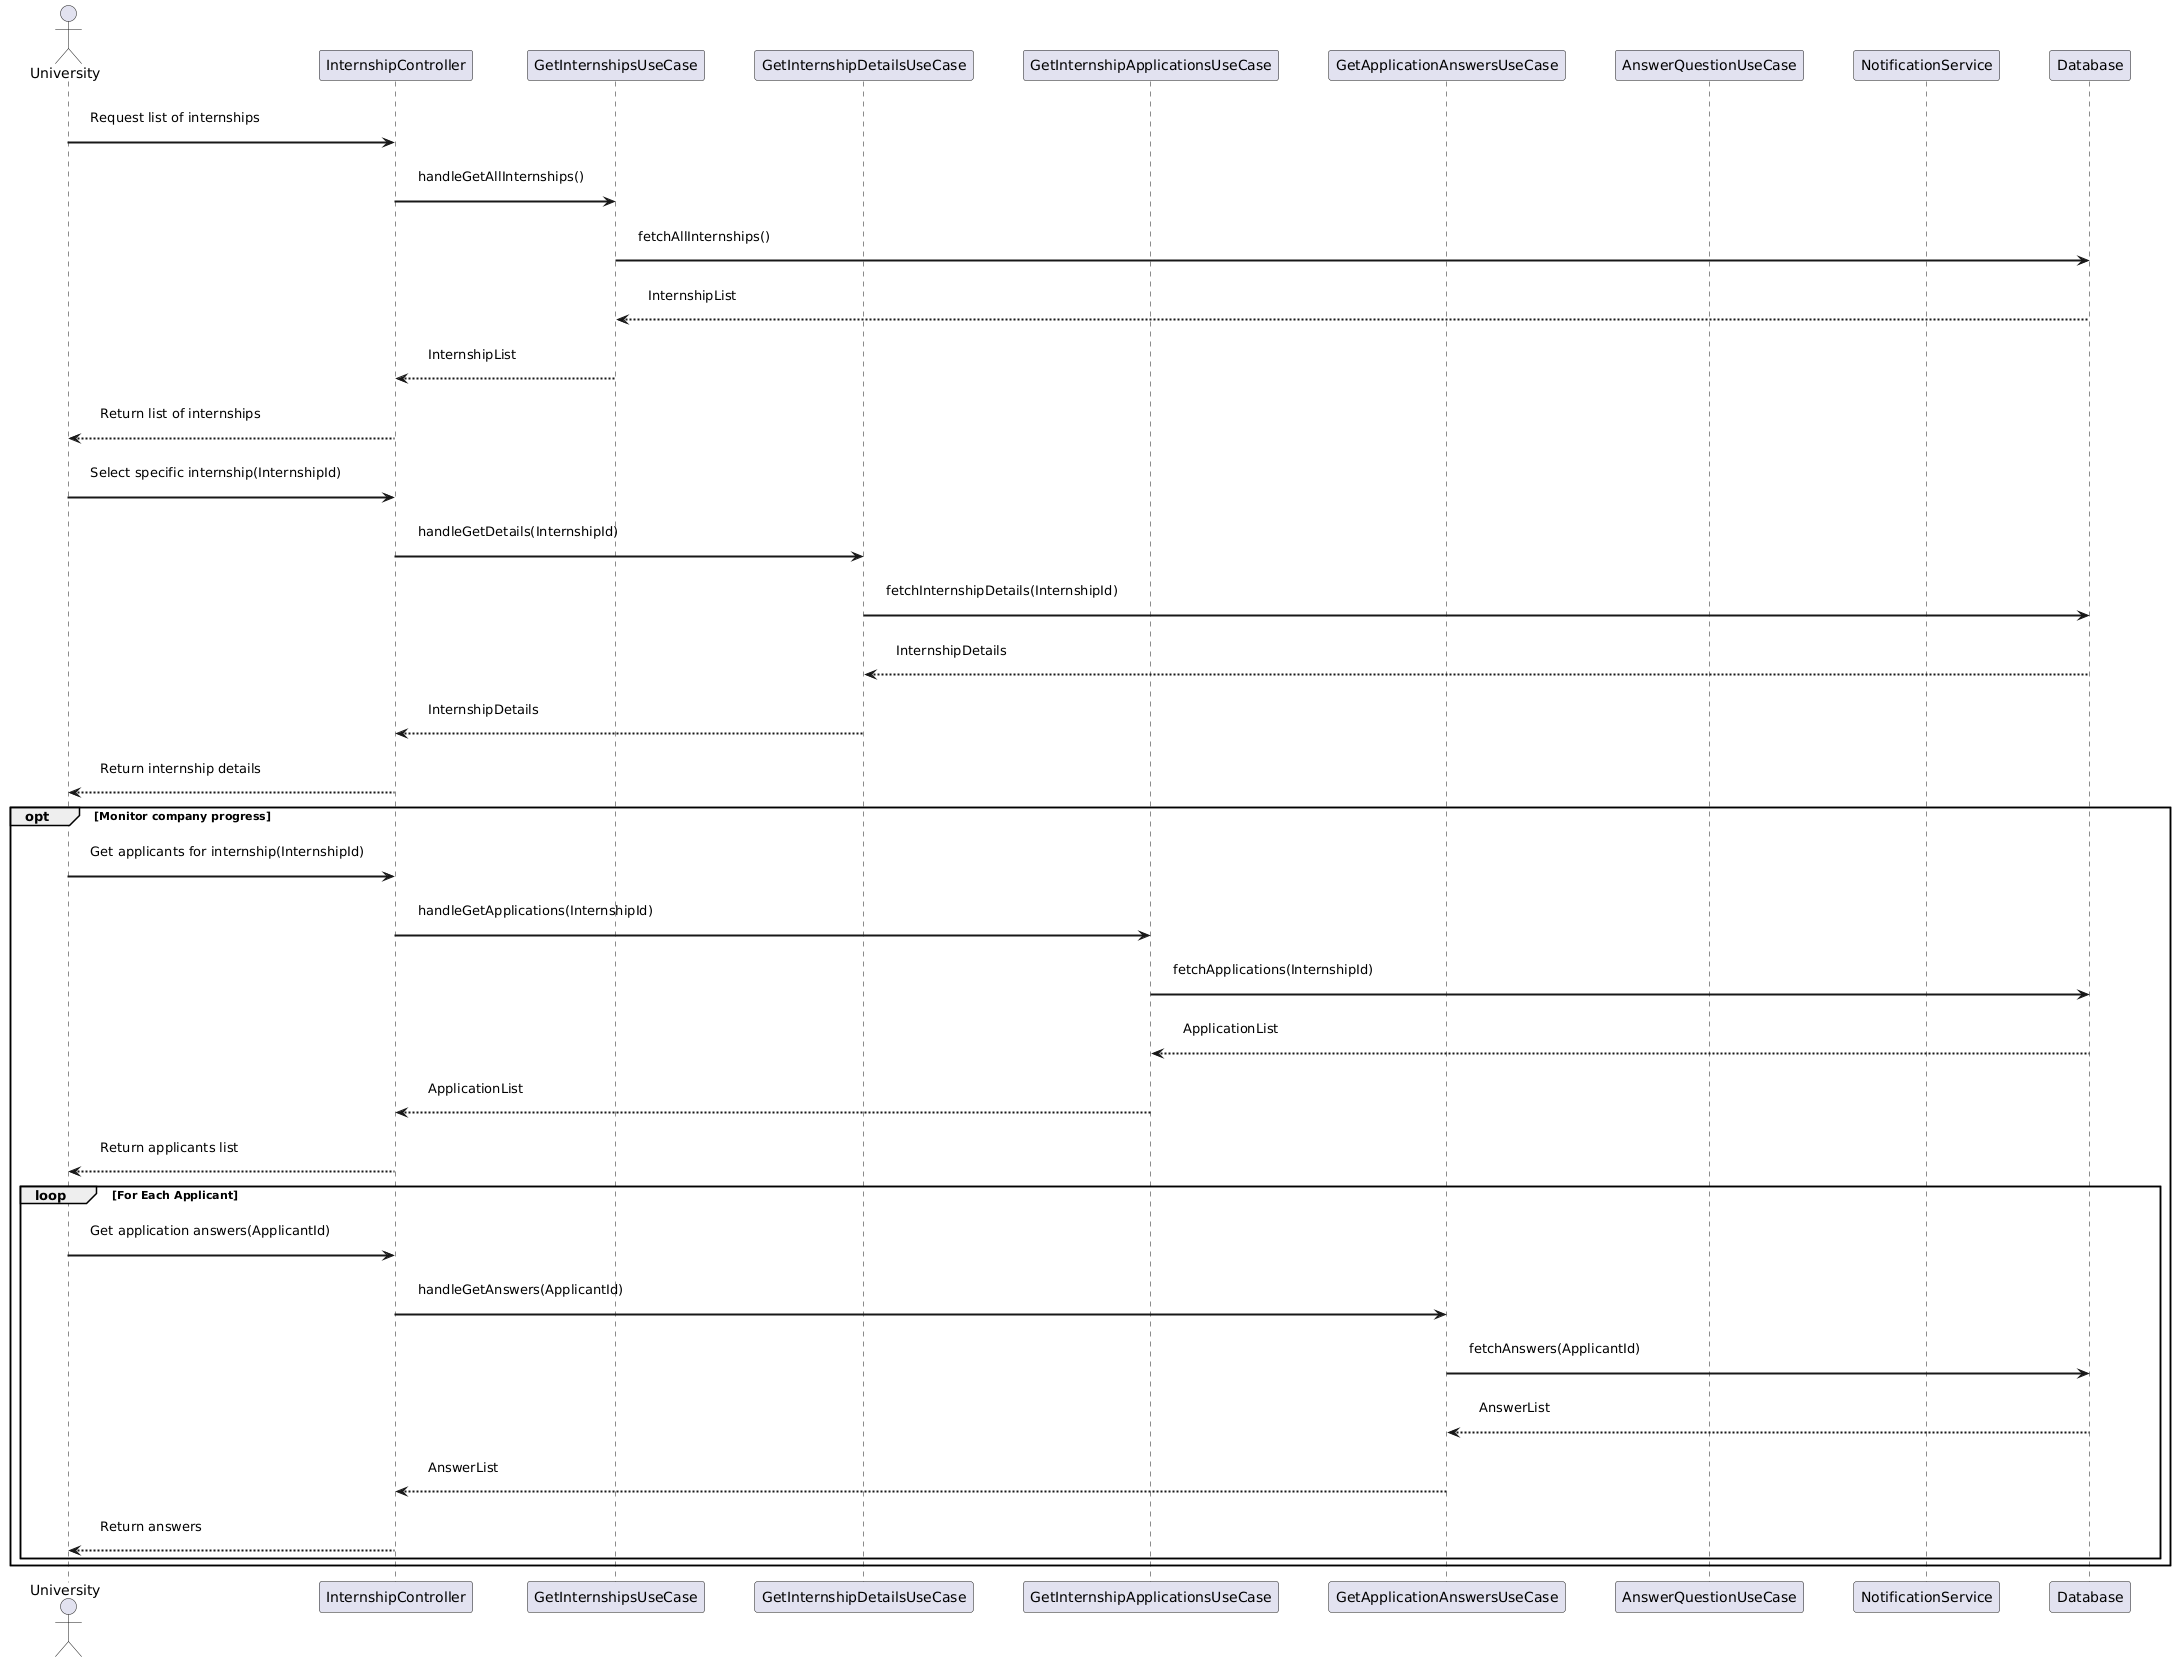
\includegraphics[scale=0.21]{Images/ImagesSequenceDiagram/UniversityMonitorsInternship.png}
    \caption{University monitors the progress of internships}
\end{figure}

\newpage

\section{Component interfaces}

In this section we use the word \textbf{"Dto"} referring to a datatype defined in the backend containing all the required attribute. The input taken from the frontend or the output coming from the backend are mapped into a dto to double check the correctness of the values.

\begin{itemize}
\item \textbf{Authentication}
Handles all processes related to user authentication, such as logging in, logging out, token refreshment, and password management.

\begin{itemize}
    \item \textbf{register(dto: RegisterDto): TokenResponse} – Registers a new user (student, company or university) by saving the provided data and returns a \textit{TokenResponseDto}.
    \item \textbf{login(email: string, password: string): TokenResponseDto} – Authenticates a user (student or company) by validating credentials. If successful, returns a \textit{TokenResponseDto}.
    \item \textbf{logout(): void} – Logs out the user, ending their session.
    \item \textbf{refreshToken(refreshToken: String): TokenResponse} – Extends the session duration by generating a new \textit{authToken} if the refresh token is valid.
    \item \textbf{resetPasswordRequest(email: String): void} – Sends a password reset link to the provided email, allowing users to initiate the password reset process.
    \item \textbf{resetPassword(token: String, newPassword: String): Bool} – Validates the reset token sent to the user's email and updates the password if the token is valid. Returns \textit{true} upon success.
    \item \textbf{verifyEmail(verifyEmail: VerifyEmailDto): VerifyResponse} - verify the email validity.
    \item \textbf{sendVerificationEmail(sendVerify: SendVerificationDto): void} - end the verification email after the registration.
\end{itemize}

\item \textbf{Internship}

\begin{itemize}
\item \textbf{getInternship() : List<InternshipDto> } - Allows platform to retrieve all the internship to fill the homepage.
    \item \textbf{createInternship(companyId: ID, internshipData: Internship): ID} – Allows a company to create a new internship posting, returning the ID of the new internship.
    \item \textbf{applyToInternship(studentId: int, internshiptId: int): ApplicationDto} - Send the student application to a specific internship.
    \iterm \textbf{getInternshipApplicants(internshipId: int, companyId: int): List<StudentDto>} - Retrieves the student that had applied for an internship of a company.
    \item \textbf{updateStatusApplication(applicationId: int, updatedStatus:updatedStatusApplicationDto, companyId: int  ): ApplicationDto} – Updates an existing application changing its status.
    \item \textbf{answerApplicationQuestions(applicationId: int, answer: AnswerQuestionsDto, studentId: int} - Add the student's answers to the application.
    \item \textbf{deleteInternship(internshipId: int): void} – Deletes an internship listing, making it inactive or removing it from the view.
\end{itemize}



\item \textbf{Student}
The Student Controller manages requests related to student profiles, such as updates and viewing application history.

\begin{itemize}
    \item \textbf{getStudent(studentId: int): void} – Get the student profile.
    \item \textbf{updateStudentProfile(studentId: ID, updatedData: UpdateStudentDto): void} – Allows a student to update their profile with new information, such as contact details or academic information.
    \item \textbf{loadCvStudent(dto: LoadCvDto, studentId: int): CvDto}
    \item \textbf{listStudentApplications(studentId: int): List<Application>} – Returns the history of internship applications made by the student.
\end{itemize}

\item \textbf{Match}
The match controller manages finding and retrieving the matches between the company's internship suitable skills and the students' one.
\begin{itemize}

    \item \textbf{GetStudentMatches(studentId: int): List<MatchDto>} - Retrieve the student matches with the intenship of various companies.
    \item \textbf{GetCompanyMathes(companyId: int): List<MatchDto} - Retrieve the company matches between the suitable skills of the students and of their internships.
    \item \textbf{inviteStudent(matchId: int, companyId: int): void} - Company invite a student who is matching with one of its internship.
    \item \textbf{acceptMatch(matchId: int, studentId: int): void} - Student accept one of the invite sent by the company.

\end{itemize}


\item \textbf{Feedback}
The Feedback Controller manages operations for collecting and handling feedback within the system.

\begin{itemize}
    \item \textbf{submitFeedback(userId: ID, internshipId: ID, feedbackData: Feedback): void} – Allows a user (student or company) to submit feedback on an internship or application experience.
    \item \textbf{getFeedbackForInternship(internshipId: ID): List<Feedback>} – Retrieves all feedback associated with a specific internship, useful for administrators to monitor feedback trends.
    \item \textbf{getFeedbackForStudent(studentId: ID): List<Feedback>} – Retrieves feedback given to or by a student, allowing administrators to track individual experiences.
\end{itemize}

\item \textbf{Company}
The Company Controller is responsible for managing company accounts and interaction with internship postings and applications.

\begin{itemize}
    \item \textbf{getProfile(comapanyId: int): CompanyDto} – Creates a new company profile and returns the company ID.
    \item \textbf{updateCompanyProfile(companyId: int, updatedData: CompanyDto): void} – Allows a company to update its profile information, such as contact details or industry.
    \item \textbf{getInternships(companyId: int): List<Internship>} – Lists all internships posted by the company.
    \item \textbf{addInternship(companyId: int, updateData: InternshipDto): void} - Add an internship.
    \item \textbf{updateInternship(companyId: int, internshipId: int, updateData: InternshipUpdateDto): void} - Update a current internship of a company.
    \item \textbf{getQuestions(companyId: int)} - Get the questions created by the companies.
    \item \textbf{addQuestion(companyId: int, updateQuestion: UpdateQuestionDto} - Add a new question.
    \item \textbf{acceptApplication(companyId: int, applicationId: int): void} – Allows a company to accept a student application for an internship.
    \item \textbf{rejectApplication(companyId: int, applicationId: int): void} – Allows a company to reject a student application for an internship.
\end{itemize}

\item \textbf{University}
The university controller is used to manage the university's interactions with students' internships and feedback.
\begin{itemize}
    \item \textbf{getStudentInternshipRecords(studentId: ID): List<Internship>} – Retrieves a list of internships a student has participated in, including completed and current ones.
    \item \textbf{collectFeedback(studentId: ID, internshipId: ID): Feedback} – Collects feedback from students regarding their internship experience for quality assurance and improvement.
    \item \textbf{assignInternshipAdvisor(studentId: ID, advisorId: ID): void} – Assigns an academic advisor to a student's internship to provide guidance and support.
    \item \textbf{listAllFeedback(internshipId: ID): List<Feedback>} – Returns all feedback related to a specific internship to assess overall satisfaction and outcomes.
    \item \textbf{getInternshipApprovalStatus(studentId: ID, internshipId: ID): ApprovalStatus} – Retrieves the current approval status for a student's internship application.
    \item \textbf{updateStudentFeedback(studentId: ID, feedbackId: ID, updatedFeedback: Feedback): void} – Updates feedback provided by a student if changes are needed.
\end{itemize}



\newpage

\end{itemize}


\section{Selected architectural styles and patterns}
\textbf{Monolithic server:} 
We chose a monolithic approach for its simplicity, faster development, and easier management. It minimizes the complexities of inter-service communication and ensures consistent control, which is ideal for smaller teams or projects with limited resources. This approach also offers better performance and simpler security management, making it a practical choice for our project’s scope

\textbf{Fat client:}
Fat clients allow offering a wide variety of functionalities independent from the central server, as well as to move part of the business logic off of the server and into the clients. The main advantages it offers are greater decoupling of frontend and backend as well as a better interactive experience, especially in conditions where the client is on an unstable network. Additionally, with the adoption of a single-page applications, there are many cross-platform frameworks which allow to reuse code partially or entirely on multiple platforms. The single-page web application can also be served by a dedicated static web server, as all its interactivity is implemented client-side, further reducing the burden on the server by delegating its serving to a CDN, which is highly optimized for
this specific use case.

\textbf{REST API:}
An architectural style defined on top of HTTP centered around the definition of a standardized set of stateless operations. Its main advantages are its simplicity, its use of widely adopted standards which facilitate adoption, and its ease of scalability given by its stateless nature. It allows to have a single API interface against which a heterogeneous set of clients can make requests.

\textbf{Component-based architecture:}
In the frontend, we have focused on a component-based architecture. This approach structures the application as a collection of reusable and self-contained components, each managing its logic, rendering, and state. By adopting this architecture, we ensure that the code is modular, making it easier to maintain, update. Reusability is a key advantage, as components can be composed and reused across different sections of the app, leading to more efficient development and consistent user interfaces.


\section{Other design decisions}

\textbf{Relational DBMS}: 
We chose to integrate a Database Management System (DBMS) into our project to ensure efficient data management, storage, and retrieval. A DBMS provides a structured and scalable way to handle large volumes of data while maintaining data integrity, consistency, and security. It allows for multi-user access, concurrent data manipulation, and facilitates complex queries that enhance the project's functionality and performance. The choice of a DBMS also supports data backup and recovery, reducing the risk of data loss and ensuring system reliability. Overall, it is an essential component for building a robust, reliable, and scalable solution


\chapter{User interface design}
\section{Student Flows}

\subsection{Student Registration/Login and First Job Application Flow}
\begin{itemize}
    \item Students register by providing email, password, and selecting the profile type (\texttt{Student}).
    \item Students fill their personal info before applying to any job.
    \item Students browse job postings.
    \item Applications are confirmed upon submission, and students can track their status.
\end{itemize}

\subsection{Matches Flow}
\begin{itemize}
    \item Students can review invitations from companies and explore job suggestions provided by the application tool.
    \item Students have the option to select a suitable job from the suggested matches and proceed with the application process.
\end{itemize}

\subsection{Application Status and Feedback Flow}
\begin{itemize}
    \item Jobs requiring assessments allow students to submit responses to:
    \begin{itemize}
        \item Open-ended questions.
        \item Multiple-choice questions.
        \item True/False questions.
    \end{itemize}
    \item Students monitor the status of applications.
    \item Students can exchange feedback on Ongoing Jobs.
    \item Students can exchange feedback about the platform.
\end{itemize}
\newpage
\section{Company Flows}

\subsection{Company Registration/Login and Job Creation Flow}
\begin{itemize}
    \item Companies register by providing email, password, and selecting the profile type (\texttt{Company}).
    \item Companies fill their personal info before creating any job.
    \item Companies create jobs by providing:
    \begin{itemize}
        \item Title, location, deadline, description, job type, and required skills.
    \end{itemize}
    \item Additional questions (open-ended, multiple choice, true/false) can be added to applications.
    \item A list of posted jobs is available for management and tracking.
\end{itemize}

\subsection{Candidate Matching and Invitation Flow}
\begin{itemize}
    \item Matches suggest suitable candidates for listed jobs.
    \item Invitations are sent to candidates.
\end{itemize}

\subsection{Application Review Flow}
\begin{itemize}
    \item Companies review applications.
    \item Applicants’ details, including CV and skills, are displayed alongside submission dates and informations depending on the status.
    \item Applications can be accepted or rejected.
    \item Companies can add feedback on Ongoing jobs.
\end{itemize}

\section{University Flows}

\subsection{University Interaction Flow}
\begin{itemize}
    \item Universities oversee the activities of their students, ensuring proper monitoring and progress tracking.
    \item Universities have access to detailed information about students, job roles, and their current statuses.
    \item Universities can send notifications to both students and companies to communicate important updates or deadlines.
    \item Universities can review feedback provided by both companies and students to ensure transparency and accountability.
\end{itemize}

\includepdf[pages=1, pagecommand={%
    \begin{tikzpicture}[overlay, remember picture]
        \draw[red, ultra thick] (13.5cm, 3.5cm) rectangle (15.5cm, 2.5cm);
        \node[red] at (14.5cm, 3cm) {\textbf{3.1.1}};
    \end{tikzpicture}
}]{Images/flows/StudentFlow1.pdf}
\includepdf[pages=1, pagecommand={%
    \begin{tikzpicture}[overlay, remember picture]
        \draw[red, ultra thick] (13.5cm, 3.5cm) rectangle (15.5cm, 2.5cm);
        \node[red] at (14.5cm, 3cm) {\textbf{3.1.1}};
    \end{tikzpicture}
}]{Images/flows/StudentFlow1-1.pdf}
\includepdf[pages=1, pagecommand={%
    \begin{tikzpicture}[overlay, remember picture]
        \draw[red, ultra thick] (13.5cm, 3.5cm) rectangle (15.5cm, 2.5cm);
        \node[red] at (14.5cm, 3cm) {\textbf{3.1.2}};
    \end{tikzpicture}
}]{Images/flows/StudentFlow2.pdf}
\includepdf[pages=1, pagecommand={%
    \begin{tikzpicture}[overlay, remember picture]
        \draw[red, ultra thick] (13.5cm, 3.5cm) rectangle (15.5cm, 2.5cm);
        \node[red] at (14.5cm, 3cm) {\textbf{3.1.3}};
    \end{tikzpicture}
}]{Images/flows/StudentFlow3.pdf}
\includepdf[pages=1, pagecommand={%
    \begin{tikzpicture}[overlay, remember picture]
        \draw[red, ultra thick] (13.5cm, 3.5cm) rectangle (15.5cm, 2.5cm);
        \node[red] at (14.5cm, 3cm) {\textbf{3.2.1}};
    \end{tikzpicture}
}]{Images/flows/CompanyFlow1.pdf}
\includepdf[pages=1, pagecommand={%
    \begin{tikzpicture}[overlay, remember picture]
        \draw[red, ultra thick] (13.5cm, 3.5cm) rectangle (15.5cm, 2.5cm);
        \node[red] at (14.5cm, 3cm) {\textbf{3.2.1}};
    \end{tikzpicture}
}]{Images/flows/CompanyFlow1-1.pdf}
\includepdf[pages=1, pagecommand={%
    \begin{tikzpicture}[overlay, remember picture]
        \draw[red, ultra thick] (13.5cm, 3.5cm) rectangle (15.5cm, 2.5cm);
        \node[red] at (14.5cm, 3cm) {\textbf{3.2.2}};
    \end{tikzpicture}
}]{Images/flows/CompanyFlow2.pdf}
\includepdf[pages=1, pagecommand={%
    \begin{tikzpicture}[overlay, remember picture]
        \draw[red, ultra thick] (13.5cm, 3.5cm) rectangle (15.5cm, 2.5cm);
        \node[red] at (14.5cm, 3cm) {\textbf{3.2.3}};
    \end{tikzpicture}
}]{Images/flows/CompanyFlow3.pdf}
\includepdf[pages=1, pagecommand={%
    \begin{tikzpicture}[overlay, remember picture]
        \draw[red, ultra thick] (13.5cm, 3.5cm) rectangle (15.5cm, 2.5cm);
        \node[red] at (14.5cm, 3cm) {\textbf{3.2.3}};
    \end{tikzpicture}
}]{Images/flows/CompanyFlow3-1.pdf}
\includepdf[pages=1, pagecommand={%
    \begin{tikzpicture}[overlay, remember picture]
        \draw[red, ultra thick] (13.5cm, 3.5cm) rectangle (15.5cm, 2.5cm);
        \node[red] at (14.5cm, 3cm) {\textbf{3.3.1}};
    \end{tikzpicture}
}]{Images/flows/UniversityFlow1.pdf}

\chapter{Requirements traceability}
\begin{longtable}{|p{3cm}|p{5cm}|p{4cm}|}
\hline
\textbf{Requirements} & \textbf{Description} & \textbf{Components} \\
\hline

R9, R10 & Allow students to view internship recommendations and trends. & Student Controller \\
\hline
R5, R6 & Allow students to create/edit profiles, upload CVs, and receive validation. & Student Controller \\
\hline
R8, R19 & Provide a search tool with filtering options for internships. & Student Controller, Internship Controller \\
\hline
R12, R18 & Guide students through the application process and track application statuses. & Student Controller, Internship Controller \\
\hline
R15, R16, R28, R29 & Companies can create, edit, and manage internship postings with deadlines, and various criteria. & Company Controller, Internship Controller \\
\hline
R17, R20 & Enable companies to access ad hoc pages for reviewing applications and analyzing applicants. & Company Controller \\
\hline
R19, R9 & Provide a recommendation feed for companies to find candidates and view suitable profiles. & Company Controller, Internship Controller, Match Controller \\
\hline
R24, R25 & Universities can monitor internship progress, manage complaints, and track student engagement. & Internship Controller, Feedback Controller \\
\hline
R26, R27 & Integrate securely with university databases and external platforms for data verification and feedback collection. & Internship Controller, Feedback Controller \\
\hline
R10, R9 & Improve recommendation engine and notify students of suitable internship. & Internship Controller, Student Controller \\
\hline
R16, R21 & Allow companies to manage interview schedules and outcomes, including feedback to the platform. & Company Controller, Feedback Controller \\
\hline
R22, R23 & Collect and display post-internship feedback and endorsements. & Feedback Controller \\
\hline
R1, R2, R3 & Implement security measures to the login and registration of the account. & Authentication Controller \\
\hline
R23 & Display top-rated internships based on feedback. & Feedback Controller, Internship Controller \\
\hline
R7 & Assessment tool for answering the application answers. & Student Controller \\
\hline
R10, R19 & Rank and score internship recommendations for students. & Internship Controller, Match Controller \\
\hline
\end{longtable}


\chapter{Implementation, integration and test plan}
In this section, we outline the implementation strategy, the integration methodology, and the comprehensive testing plan for the job boarding web application, developed using React for the frontend and ASP.NET Core as a monolithic server for the backend. The architecture chosen ensures high decoupling of code, primarily facilitated by dependency injection.

\subsection{Development Plan}

The development process will follow a bottom-up approach, focusing on the incremental building of backend components and simultaneous development of the frontend. The backend is structured into multiple sections, each serving a distinct purpose and responsible for various features. The key features to be developed are as follows:

\begin{itemize}
    \item \textbf{Authentication Management}: Manages user registration, login, and session handling. It is foundational, as most other features depend on authenticated access.
    \item \textbf{Student Information Management}: Handles CRUD operations for student profiles, including their personal details, resumes, and application history.
    \item \textbf{Company Information Management}: Supports company profiles
    \item \textbf{Internship Management}: Manages internship postings, applications, and status updates.
    \item \textbf{Matching Management}: Manages matching processes and recommendation improving system.
    \item \textbf{Feedback Management}: Manages the feedback system that guarantees students and companies to provide feedbacks on the platform and on companies(for students) and students(for companies)  .
\end{itemize}

Each feature will be developed in sequence, respecting dependencies (e.g., the Authentication Module must be implemented before Student and Company Information Management). Development will be conducted alongside unit testing for each component to ensure correctness and stability. Additionally, testing of the backend functionalities is performed using Postman to validate API endpoints, ensure expected behavior, and facilitate the later integration with the frontend components.

\subsection{Component Integration and Testing}

Once individual components are developed and unit tested, the integration phase begins. Integration will be performed in stages:

\begin{itemize}
    \item \textbf{Phase 1: Backend Integration}: Integrate and communicate between the several backend sections developed.
    \item \textbf{Phase 2: Backend-Frontend Integration}: Connect the frontend React application to the backend API endpoints. This step involves verifying that data requests and responses between the client and server are functioning as intended.
\end{itemize}

During this phase, integration tests will be conducted to verify that the combined components function as expected when communicating with each other.

\subsection{System and End-to-End (E2E) Testing}

Once all components have been successfully integrated, system testing will be conducted to ensure that the complete solution functions cohesively. This phase focuses on verifying that all integrated components interact correctly and perform as expected in a unified environment. System testing will comprehend the following type of tests:

\begin{itemize}
\item \textbf{Load Testing}: Assess the system's ability to handle varying levels of user traffic and operational demands, ensuring stability under stress. \item \textbf{Performance Testing}: Measure the system's response times and performance metrics under both typical and peak usage conditions to ensure reliability and scalability.
\end{itemize}

End-to-End (E2E) testing will simulate real user interactions with the application through the frontend interface, validating the application's functionality, workflow, and overall behavior from start to finish.



\subsection{Acceptance Testing}

The final phase of testing is acceptance testing, which involves stakeholders and representative users. This testing stage is crucial to ensure that the system meets the business requirements and user expectations. Once a beta version of the software is available, the acceptance testing process will proceed as follows:

\begin{itemize}
    \item \textbf{User-Based Scenarios}: Real users, including stakeholders, will perform typical tasks on the system (e.g., creating an account, browsing job postings, and applying for internships).
    \item \textbf{Feedback Collection}: User feedback will be gathered to identify usability issues, missing features, or areas for improvement.
    \item \textbf{Validation}: Confirm that the system meets the acceptance criteria defined in the project requirements.
\end{itemize}

Acceptance testing will conclude with a review meeting, where results and feedback are discussed, leading to necessary adjustments before the final release.


\chapter{Effort spent}
\section{Effort Spent}

\begin{table}[ht!]
\centering
\renewcommand{\arraystretch}{1.6}
\begin{tabular}{|c|l|c|}
\hline
\textbf{Member of Group} & \textbf{Effort Spent} & \textbf{Hours} \\ \hline
\multirow{5}{*}{Giovanni Vaccarino} 
    & Introduction & 2h \\ \cline{2-3}
    & Overall Description & 1h \\ \cline{2-3}
    & Specific Requirements & 3h \\ \cline{2-3}
    & Formal Analysis & 1h \\ \hline
\multirow{5}{*}{Vittorio Palladino} 
    & Introduction & 2h \\ \cline{2-3}
    & Overall Description & 1h \\ \cline{2-3}
    & Specific Requirements & 1h \\ \cline{2-3}
    & Formal Analysis & 4h \\ \hline
\multirow{5}{*}{Nicolò Vacis} 
    & Introduction & 1h \\ \cline{2-3}
    & Overall Description & 3h \\ \cline{2-3}
    & Specific Requirements & 2h \\ \cline{2-3}
    & Formal Analysis & 1h \\ \hline
\end{tabular}
\caption{Effort spent by each member of the group}
\end{table}


\chapter{References}
\section{References}
\begin{itemize}
    \item 2024-2025 Software Engineering 2 - Assignment RASD
\end{itemize}


\cleardoublepage

\end{document}
